% Options for packages loaded elsewhere
\PassOptionsToPackage{unicode}{hyperref}
\PassOptionsToPackage{hyphens}{url}
\documentclass[
  11pt,
]{article}
\usepackage{xcolor}
\usepackage[left=3cm,right=3cm,top=2.5cm,bottom=2.5cm]{geometry}
\usepackage{amsmath,amssymb}
\setcounter{secnumdepth}{5}
\usepackage{iftex}
\ifPDFTeX
  \usepackage[T1]{fontenc}
  \usepackage[utf8]{inputenc}
  \usepackage{textcomp} % provide euro and other symbols
\else % if luatex or xetex
  \usepackage{unicode-math} % this also loads fontspec
  \defaultfontfeatures{Scale=MatchLowercase}
  \defaultfontfeatures[\rmfamily]{Ligatures=TeX,Scale=1}
\fi
\usepackage{lmodern}
\ifPDFTeX\else
  % xetex/luatex font selection
\fi
% Use upquote if available, for straight quotes in verbatim environments
\IfFileExists{upquote.sty}{\usepackage{upquote}}{}
\IfFileExists{microtype.sty}{% use microtype if available
  \usepackage[]{microtype}
  \UseMicrotypeSet[protrusion]{basicmath} % disable protrusion for tt fonts
}{}
\usepackage{setspace}
\makeatletter
\@ifundefined{KOMAClassName}{% if non-KOMA class
  \IfFileExists{parskip.sty}{%
    \usepackage{parskip}
  }{% else
    \setlength{\parindent}{0pt}
    \setlength{\parskip}{6pt plus 2pt minus 1pt}}
}{% if KOMA class
  \KOMAoptions{parskip=half}}
\makeatother
\usepackage{longtable,booktabs,array}
\usepackage{caption}
\captionsetup[table]{skip=6pt}
\newcounter{none} % for unnumbered tables
\usepackage{calc} % for calculating minipage widths
% Correct order of tables after \paragraph or \subparagraph
\usepackage{etoolbox}
\makeatletter
\patchcmd\longtable{\par}{\if@noskipsec\mbox{}\fi\par}{}{}
\makeatother
% Allow footnotes in longtable head/foot
\IfFileExists{footnotehyper.sty}{\usepackage{footnotehyper}}{\usepackage{footnote}}
\makesavenoteenv{longtable}
\usepackage{graphicx}
\makeatletter
\newsavebox\pandoc@box
\newcommand*\pandocbounded[1]{% scales image to fit in text height/width
  \sbox\pandoc@box{#1}%
  \Gscale@div\@tempa{\textheight}{\dimexpr\ht\pandoc@box+\dp\pandoc@box\relax}%
  \Gscale@div\@tempb{\linewidth}{\wd\pandoc@box}%
  \ifdim\@tempb\p@<\@tempa\p@\let\@tempa\@tempb\fi% select the smaller of both
  \ifdim\@tempa\p@<\p@\scalebox{\@tempa}{\usebox\pandoc@box}%
  \else\usebox{\pandoc@box}%
  \fi%
}
% Set default figure placement to htbp
\def\fps@figure{htbp}
\makeatother
% definitions for citeproc citations
\NewDocumentCommand\citeproctext{}{}
\NewDocumentCommand\citeproc{mm}{%
  \begingroup\def\citeproctext{#2}\cite{#1}\endgroup}
\makeatletter
 % allow citations to break across lines
 \let\@cite@ofmt\@firstofone
 % avoid brackets around text for \cite:
 \def\@biblabel#1{}
 \def\@cite#1#2{{#1\if@tempswa , #2\fi}}
\makeatother
\newlength{\cslhangindent}
\setlength{\cslhangindent}{1.5em}
\newlength{\csllabelwidth}
\setlength{\csllabelwidth}{3em}
\newenvironment{CSLReferences}[2] % #1 hanging-indent, #2 entry-spacing
 {\begin{list}{}{%
  \setlength{\itemindent}{0pt}
  \setlength{\leftmargin}{0pt}
  \setlength{\parsep}{0pt}
  % turn on hanging indent if param 1 is 1
  \ifodd #1
   \setlength{\leftmargin}{\cslhangindent}
   \setlength{\itemindent}{-1\cslhangindent}
  \fi
  % set entry spacing
  \setlength{\itemsep}{#2\baselineskip}}}
 {\end{list}}
\usepackage{calc}
\newcommand{\CSLBlock}[1]{\hfill\break\parbox[t]{\linewidth}{\strut\ignorespaces#1\strut}}
\newcommand{\CSLLeftMargin}[1]{\parbox[t]{\csllabelwidth}{\strut#1\strut}}
\newcommand{\CSLRightInline}[1]{\parbox[t]{\linewidth - \csllabelwidth}{\strut#1\strut}}
\newcommand{\CSLIndent}[1]{\hspace{\cslhangindent}#1}
\setlength{\emergencystretch}{3em} % prevent overfull lines
\providecommand{\tightlist}{%
  \setlength{\itemsep}{0pt}\setlength{\parskip}{0pt}}
% Paragraph scaffolding for manuscript revision.
%
% Two environments, presented in this order per paragraph:
%
%   rgt   -- author's rewrite (initially a placeholder)
%            small, italic, dark blue
%   orig  -- original Claude-authored draft, and until the rewrite
%            replaces it, the body text of the manuscript
%            normal size, gray
%
% The `bullets' environment (a boiled-down topic sentence plus bullet
% points, one per paragraph) is no longer used inside manuscripts:
% those blocks now live in a companion bullets.Rmd supplement in the
% same report directory, which typesets them as plain \textbf{} +
% itemize and needs no part of this file. The definition is retained
% only so that a stray block left in a document still compiles.
%
% This file is identical across every manuscript that includes it.
% It previously existed in two variants that swapped the sizes of
% rgt and orig, so the same markup rendered differently depending on
% which repository the manuscript lived in. The variant retained here
% keeps orig at full size because orig, not rgt, currently carries
% the prose in every manuscript in the pool.

\usepackage{xcolor}

\newcounter{pgraph}

\newenvironment{bullets}{%
  \stepcounter{pgraph}%
  \begin{quote}\small\sffamily\color[gray]{0.30}%
  {\normalfont\scriptsize\color[gray]{0.58}[\thepgraph]\enspace}}{%
  \end{quote}}

\newenvironment{rgt}{%
  \begin{quote}\small\itshape\color[RGB]{20,60,160}}{%
  \end{quote}}

\newenvironment{orig}{%
  \begin{quote}\normalsize\color[gray]{0.55}}{%
  \end{quote}}

% backward compat alias
\newenvironment{claudecode}{\begin{orig}}{\end{orig}}
%% tools/stamp.tex
%% Provenance footer for PDFs rendered from this project.
%% Vendored by zzcollab; this file is not project-specific. The
%% footer prints the source document and the time of rendering.
%% The git version is defined here too, and so is available to a
%% project that wants it on the page, but it is left off the
%% default footer: it already names the staged copy in share/ and
%% appears in its manifest row. All values are supplied at render
%% time by tools/stamp-render.R, which writes a small generated
%% file that redefines the macros below. The \providecommand
%% defaults keep a bare LaTeX compile working when the document is
%% built without the wrapper.
\usepackage{fancyhdr}
\usepackage{xcolor}
\providecommand{\stampsource}{\detokenize{(source not recorded)}}
\providecommand{\stamptime}{(time not recorded)}
\providecommand{\stampversion}{\detokenize{(version not recorded)}}
\setlength{\footskip}{40pt}
\newcommand{\stampfootcontent}{%
  \footnotesize\color{gray}%
  \parbox[b]{\textwidth}{%
    \stamptime\hfill\thepage\\[2pt]%
    \ttfamily\raggedright\stampsource}}
\pagestyle{fancy}
\fancyhf{}
\fancyfoot[C]{\stampfootcontent}
\renewcommand{\headrulewidth}{0pt}
\renewcommand{\footrulewidth}{0.4pt}
%% The title page uses the `plain` page style; redefine it so the
%% stamp appears there too.
\fancypagestyle{plain}{%
  \fancyhf{}%
  \fancyfoot[C]{\stampfootcontent}%
  \renewcommand{\headrulewidth}{0pt}%
  \renewcommand{\footrulewidth}{0.4pt}}
\renewcommand{\stampsource}{\textasciitilde{}/\allowbreak{}prj/\allowbreak{}res/\allowbreak{}36-pmsimstats-ng/\allowbreak{}pmsimstats-ng/\allowbreak{}analysis/\allowbreak{}report/\allowbreak{}05-nof1-design-sensitivity/\allowbreak{}report.Rmd}
\renewcommand{\stamptime}{2026-08-15 16:50 PDT}
\renewcommand{\stampversion}{\detokenize{bc0b671-wip}}
\usepackage{amsmath}
\usepackage{amssymb}
\usepackage{booktabs}
\usepackage{longtable}
\usepackage{float}
\usepackage[mathlines]{lineno}
\linenumbers
\usepackage{bookmark}
\IfFileExists{xurl.sty}{\usepackage{xurl}}{} % add URL line breaks if available
\urlstyle{same}
% fallback for those not using the hyperref driver hyperxmp:
\makeatletter
\@ifundefined{xmpquote}{\newcommand{\xmpquote}[1]{#1}}{}
\makeatother
\hypersetup{
  pdftitle={Power sensitivity of a hybrid open-label-plus-blinded- discontinuation N-of-1 design under carryover{,} serial correlation{,} and variance-component variation},
  pdfauthor={pmsimstats team},
  hidelinks,
  pdfcreator={LaTeX via pandoc}}

\title{Power sensitivity of a hybrid open-label-plus-blinded- discontinuation N-of-1 design under carryover, serial correlation, and variance-component variation}
\author{pmsimstats team}
\date{August 15, 2026}

\begin{document}
\maketitle

{
\setcounter{tocdepth}{2}
\tableofcontents
}
\setstretch{1.1}
\section{Abstract}\label{abstract}

\textbf{Background.} Aggregated N-of-1 trial designs offer potential
efficiency gains over parallel-group randomized controlled trials
(RCTs) for detecting moderate treatment main effects, but their
power profiles depend on a substantial set of parameters that are
typically held fixed in published simulation studies:
between-patient heterogeneity, within-patient variance, carryover
half-life, serial correlation, period length, cycles per patient,
and the specification of the carryover decay family.

\textbf{Methods.} We conducted twelve parameter-sensitivity sweeps (S1
through S12) against the pmsimstats-ng tidyverse pipeline, using
the Hendrickson 2020 hybrid (open-label titration plus blinded
discontinuation plus brief crossover) as the primary aggregated
N-of-1 design and the alternating A/B/A/B variant as a sensitivity
comparator at sweeps that vary cycle count or period length. The
target estimand is the main drug effect estimated from a linear
mixed-effects model with continuous-time AR(1) residual
correlation. Each sweep records per-replicate results so that
Monte Carlo standard errors (MCSE) can be computed at render time
per Morris et al.\textsuperscript{\citeproc{ref-morris2019simulation}{1}}.

\textbf{Results.} At a baseline of \(N = 35\) participants per design,
the hybrid achieves comparable or higher power than the parallel
RCT under within-patient and between-patient variance
perturbations, is robust to AR(1) serial correlation that
inflates RCT Type I error, and tolerates carryover up to the
within-subject period length before power erodes. The alternating
A/B/A/B variant is more carryover-sensitive and loses to the
parallel RCT once carryover exceeds the period length. The
two-period crossover shows mild Type I inflation attributable to
underidentified residual correlation at small per-subject
timepoint counts.

\textbf{Conclusions.} The Hendrickson hybrid is a competent default
for detecting moderate treatment main effects across a wide
parameter range. Design ordering becomes parallel-RCT-favored
only when carryover exceeds the within-subject period length, and
is directionally different for biomarker-treatment interaction
targets, which favor N-of-1 designs more strongly.

\textbf{Keywords.} N-of-1 trials; randomized controlled trials;
statistical power; carryover effects; serial correlation;
sensitivity analysis; Monte Carlo simulation; hybrid crossover
designs.

\section{Introduction}\label{introduction}

\begin{rgt}
Lorem ipsum dolor sit amet, consectetur adipiscing elit, sed do eiusmod tempor incididunt ut labore et dolore magna aliqua.

\end{rgt}

\begin{orig}
Aggregated N-of-1 trial designs evaluate treatment effects within
individual patients through repeated crossover periods and combine
patient-level estimates via meta-analytic or mixed-effects
machinery to support population-level inference\textsuperscript{\citeproc{ref-lillie2011}{2},\citeproc{ref-kravitzSinglepatientNof1Trials2014}{3}}. Several recent simulation
studies have reported that aggregated N-of-1 procedures can match
or exceed the statistical power of parallel-group randomized
controlled trials (RCTs) at substantially smaller participant
counts\textsuperscript{\citeproc{ref-blackstonComparisonAggregatedNof12019}{4}--\citeproc{ref-carrozzoTwoArm2025}{6}}. The reported
magnitude of this efficiency advantage, however, varies across
studies, and the conditions under which it holds or reverses are
incompletely characterized. That is, the published literature
provides encouraging headline comparisons but relatively
sparse guidance on the parameter axes that govern the
ordering of designs.

\end{orig}

\begin{rgt}
Lorem ipsum dolor sit amet, consectetur adipiscing elit, sed do eiusmod tempor incididunt ut labore et dolore magna aliqua.

\end{rgt}

\begin{orig}
We report here a systematic parameter-sensitivity study of a
specific hybrid aggregated-N-of-1 design that combines an
open-label titration phase, a blinded discontinuation phase, and a
brief crossover phase, following the design proposed by
Hendrickson and colleagues\textsuperscript{\citeproc{ref-hendricksonOptimizing2020}{5}} for
predictive-biomarker validation in chronic neurobehavioral
conditions. The sensitivity sweeps are conducted against the
pmsimstats-ng tidyverse pipeline that operationalizes this design
in R, with three parallel comparators: an alternating A/B/A/B
aggregated N-of-1 variant, a two-period crossover, and a
parallel-group RCT. The target estimand throughout is the main
drug effect, distinguished from the biomarker-treatment
interaction examined in the original Hendrickson study and in a
separate companion paper.

\end{orig}

\begin{rgt}
Lorem ipsum dolor sit amet, consectetur adipiscing elit, sed do eiusmod tempor incididunt ut labore et dolore magna aliqua.

\end{rgt}

\begin{orig}
The motivation for a sensitivity study at this granularity is
straightforward: the published simulation comparisons typically
vary one or two parameters at a time while holding the remainder
fixed at calibration defaults, leaving open the question of which
axes actually drive the N-of-1-versus-RCT power difference. We
have endeavored to address this gap by reporting twelve sensitivity
sweeps along axes drawn from the published comparison literature:
effect size\textsuperscript{\citeproc{ref-blackstonComparisonAggregatedNof12019}{4}}, carryover
half-life\textsuperscript{\citeproc{ref-blackstonComparisonAggregatedNof12019}{4},\citeproc{ref-hendricksonOptimizing2020}{5}}, decay-form
misspecification\textsuperscript{\citeproc{ref-gaertnerCarryover2023}{7}}, between-patient
heterogeneity\textsuperscript{\citeproc{ref-sennSampleSizeConsiderations2019}{8},\citeproc{ref-zucker2010}{9}}, within-patient variance\textsuperscript{\citeproc{ref-wang2019}{10}}, cycles per patient\textsuperscript{\citeproc{ref-sennSampleSizeConsiderations2019}{8}}, total participant count\textsuperscript{\citeproc{ref-blackstonComparisonAggregatedNof12019}{4},\citeproc{ref-sennSampleSizeConsiderations2019}{8}}, AR(1) serial correlation\textsuperscript{\citeproc{ref-wang2019}{10}}, period length\textsuperscript{\citeproc{ref-wang2019}{10}}, biomarker interaction strength
crossed with data-generating process architecture\textsuperscript{\citeproc{ref-hendricksonOptimizing2020}{5}}, a carryover-by-AR(1) misspecification
factorial\textsuperscript{\citeproc{ref-gaertnerCarryover2023}{7}}, and a high-replicate null
calibration\textsuperscript{\citeproc{ref-morris2019simulation}{1}}.

\end{orig}

\begin{rgt}
Lorem ipsum dolor sit amet, consectetur adipiscing elit, sed do eiusmod tempor incididunt ut labore et dolore magna aliqua.

\end{rgt}

\begin{orig}
The clinical companion to this paper (in preparation) reports a
primary head-to-head simulation comparison at the
prazosin-calibrated baseline; the present paper extends that
comparison along twelve parameter axes for the hybrid design
family specifically.

\end{orig}

\section{Simulation design}\label{simulation-design}

\subsection{Aims}\label{aims}

We follow the ADEMP framework of Morris, White, and Crowther
(2019)\textsuperscript{\citeproc{ref-morris2019simulation}{1}}: Aims, Data-generating mechanisms,
Estimands, Methods, Performance measures. The subsections of this
Simulation design section map to these five components, although
the section headers are organized by topic rather than relabeled
to the ADEMP acronym.

\begin{rgt}
Lorem ipsum dolor sit amet, consectetur adipiscing elit, sed do eiusmod tempor incididunt ut labore et dolore magna aliqua.

\end{rgt}

\begin{orig}
The simulation study has three aims. First, to characterize the
power profile of the Hendrickson 2020 hybrid aggregated-N-of-1
design\textsuperscript{\citeproc{ref-hendricksonOptimizing2020}{5}} under systematic perturbation
of the parameter axes implicated in the published
simulation-comparison literature. Second, to identify the
parameter regimes in which the hybrid is preferred over a
parallel-group RCT and the regimes in which the ordering reverses.
Third, to verify Type I error control under null and near-null
conditions, with sufficient replication to provide MCSE below
1\% per Morris et al.\textsuperscript{\citeproc{ref-morris2019simulation}{1}}.

\end{orig}

\subsection{Pipeline}\label{pipeline}

\begin{rgt}
Lorem ipsum dolor sit amet, consectetur adipiscing elit, sed do eiusmod tempor incididunt ut labore et dolore magna aliqua.

\end{rgt}

\begin{orig}
The simulation framework is implemented in the \texttt{nof1power} R
package\textsuperscript{\citeproc{ref-hendricksonOptimizing2020}{5}} developed alongside the
pmsimstats-ng tidyverse re-implementation of the Hendrickson 2020
reference pipeline. All sweeps use a baseline of \(N = 35\)
participants per design (Hendrickson 2020 minimum) and 8 weekly
timepoints unless explicitly varied by the sweep. Per-replicate
sample size is \(N\) participants for each design under comparison;
participants are matched on the per-design count rather than on
observation total, following the convention adopted in
Blackston\textsuperscript{\citeproc{ref-blackstonComparisonAggregatedNof12019}{4}},
Hendrickson\textsuperscript{\citeproc{ref-hendricksonOptimizing2020}{5}}, and the majority of
the N-of-1 simulation-comparison literature.

\end{orig}

\subsection{Dual data-generating architectures}\label{dual-data-generating-architectures}

The pipeline supports two data-generating processes (DGP) for the
biomarker-treatment interaction:

\begin{itemize}
\tightlist
\item
  \textbf{the covariance-moderation architecture (\texttt{dgp\_architecture\ =\ "mvn"}).} The
  biomarker-bio-response interaction is encoded in the covariance
  structure of a multivariate normal (MVN) draw. On-drug timepoints
  carry correlation \texttt{c.bm} between the biomarker and the
  bio-response factor; off-drug timepoints carry \texttt{c.bm\ *\ phi(tsd)}
  with \texttt{phi} the carryover decay multiplier.
\item
  \textbf{the mean-moderation architecture (\texttt{dgp\_architecture\ =\ "mean\_moderation"}).}
  After the multivariate normal draw, bio-response values at
  on-drug timepoints are shifted by \texttt{c.bm\ *\ bm\_z\ *\ br\_sd}, where
  \texttt{bm\_z} is the standardized biomarker. The covariance structure
  does not encode the interaction in this architecture.
\end{itemize}

\begin{rgt}
Lorem ipsum dolor sit amet, consectetur adipiscing elit, sed do eiusmod tempor incididunt ut labore et dolore magna aliqua.

\end{rgt}

\begin{orig}
These two architectures produce substantively different power
profiles under carryover, as documented in\textsuperscript{\citeproc{ref-hendricksonOptimizing2020}{5}}. The two architectures are crossed
in sweep S10 below; the remaining eleven sweeps use the covariance-moderation
architecture as the default.

\end{orig}

\subsection{Response curves and carryover}\label{response-curves-and-carryover}

Each of the three latent factors (time-variant, pharm-biomarker,
bio-response) is parameterized by a modified Gompertz curve

\[y(t) = \mathrm{maxr} \cdot
  \frac{\exp(-\mathrm{disp} \cdot \exp(-\mathrm{rate} \cdot t)) -
        \exp(-\mathrm{disp})}{1 - \exp(-\mathrm{disp})}\]

\begin{rgt}
Lorem ipsum dolor sit amet, consectetur adipiscing elit, sed do eiusmod tempor incididunt ut labore et dolore magna aliqua.

\end{rgt}

\begin{orig}
evaluated at the appropriate cumulative time index. The curve
passes through the origin at \(t = 0\) and asymptotes to \texttt{maxr}.
Carryover of the bio-response component during off-drug periods
is applied recursively as \(\mu[t] = \mathrm{base}[t] +
\mu[t-1] \cdot \phi(\mathrm{tsd})\) with \(\phi\) drawn from an
extensible decay family: exponential
\(\exp(-\ln 2 \cdot t / t_{1/2})\), linear
\(\max(0, 1 - t / (2 t_{1/2}))\), Weibull
\(\exp(-(\lambda_w t)^k)\) with
\(\lambda_w = (\ln 2)^{1/k} / t_{1/2}\), or power
\(\max(0, (1 - t / (3 t_{1/2}))^p)\). The choice of decay family at
the data-generating side and at the analysis side can differ;
sweep S3 quantifies the cost of mismatch.

\textbf{Units.} Carryover half-lives \(t_{1/2}\) are quoted in \textbf{days}
throughout this paper, matching the pharmacokinetic scale of the
prazosin reference application and the day-denominated axes of the
sensitivity figures. Companion papers in this series that study the
biomarker-treatment interaction (in particular the
DGP-architecture and carryover-specification manuscripts) quote
\(t_{1/2}\) in \textbf{weeks} on the canonical grid \(\{0, 0.5, 1.0\}\).
The conversion is 1 week = 7 days, so those papers' grid corresponds
to \(\{0, 3.5, 7\}\) days here, and this paper's 3-day baseline
corresponds to approximately 0.43 weeks. Timepoints \(t\) are weekly
in both conventions.

\end{orig}

\subsection{Covariance structure and analysis}\label{covariance-structure-and-analysis}

\begin{rgt}
Lorem ipsum dolor sit amet, consectetur adipiscing elit, sed do eiusmod tempor incididunt ut labore et dolore magna aliqua.

\end{rgt}

\begin{orig}
The covariance matrix couples within-factor AR(1) autocorrelation
indexed by cumulative time, cross-factor correlation at matched
and lagged timepoints, and the biomarker-bio-response
differential correlation described above. Non-positive-definite
matrices are corrected via
\texttt{corpcor::make.positive.definite(tol = 1e-3)} with a per-cell flag
returned. The analysis model fits the \texttt{nlme::lme} linear
mixed-effects formula\textsuperscript{\citeproc{ref-pinheirobates2000}{11},\citeproc{ref-verbekemolenberghs2000}{12}}
with fixed effects
\texttt{Sx \textasciitilde{} bm + t + Dbc + bm:Dbc} (or the fallback \texttt{bm + t + bm:t}
when the drug indicator does not vary within participant), a
random intercept per participant, and \texttt{corCAR1(form = \textasciitilde{}t | ptID)}
continuous-time AR(1) residual correlation. The target of
inference is the main drug effect (the \texttt{Dbc} coefficient),
extracted by matching against the row-name set \(\{\)\texttt{Dbc}\(\}\) of
the lme summary table. Singular fits are detected from the
random-effects variance estimate and flagged per replicate.

\end{orig}

\subsection{Twelve sensitivity sweeps}\label{twelve-sensitivity-sweeps}

The twelve sweeps (S1 through S12) are specified in
\texttt{docs/sensitivity-sweep-plan-2026-04-17.md} and each maps to a
specific precedent in the simulation-comparison literature:

\begin{itemize}
\tightlist
\item
  \textbf{S1} varies the effect size by scaling the bio-response
  maximum; precedent Blackston 2019\textsuperscript{\citeproc{ref-blackstonComparisonAggregatedNof12019}{4}}.
\item
  \textbf{S2} varies the carryover half-life across nine values from
  0 to 14 days across four designs (parallel RCT, two-period
  crossover, aggregated N-of-1, hybrid); precedents Blackston
  2019 and Hendrickson 2020\textsuperscript{\citeproc{ref-hendricksonOptimizing2020}{5}}.
\item
  \textbf{S3} varies the DGP carryover decay form (exponential,
  linear, Weibull, power) while the analysis assumes
  exponential, quantifying misspecification bias; precedent
  Gärtner 2023\textsuperscript{\citeproc{ref-gaertnerCarryover2023}{7}}.
\item
  \textbf{S4} varies between-patient heterogeneity via the
  baseline-symptom SD; precedents Senn 2018\textsuperscript{\citeproc{ref-sennSampleSizeConsiderations2019}{8}} and Zucker 2010\textsuperscript{\citeproc{ref-zucker2010}{9}}.
\item
  \textbf{S5} varies the within-patient bio-response SD; precedent
  Wang and Schork 2019\textsuperscript{\citeproc{ref-wang2019}{10}}.
\item
  \textbf{S6} varies the number of cycles per patient \(k\) in the
  Senn decomposition; precedent Senn 2018\textsuperscript{\citeproc{ref-sennSampleSizeConsiderations2019}{8}}.
\item
  \textbf{S7} varies the total number of participants for fixed
  cycles; precedent Senn 2018 and Blackston 2019.
\item
  \textbf{S8} varies the AR(1) correlation parameter \(\rho\) across
  within-factor autocorrelations; precedent Wang and Schork
  2019\textsuperscript{\citeproc{ref-wang2019}{10}}.
\item
  \textbf{S9} crosses period length with carryover half-life,
  probing the ratio \(t_{1/2} / \mathrm{period}\); precedent Wang
  and Schork 2019\textsuperscript{\citeproc{ref-wang2019}{10}}.
\item
  \textbf{S10} varies the biomarker interaction strength \texttt{c.bm}
  across four levels crossed with both DGP architectures (mvn,
  mean\_moderation); precedent Hendrickson 2020\textsuperscript{\citeproc{ref-hendricksonOptimizing2020}{5}}.
\item
  \textbf{S11} crosses carryover presence with AR(1) presence under
  null and alternative, to test Type I error control and power
  under DGP-analysis mismatch; precedent Gärtner 2023 and
  Blackston 2019.
\item
  \textbf{S12} is a null-effect calibration (\(c_{bm} = 0\)) at four
  \((\tau, \sigma, t_{1/2})\) configurations with 2,000
  replicates per cell for MCSE near 0.5\%; precedent Morris
  2019\textsuperscript{\citeproc{ref-morris2019simulation}{1}}.
\end{itemize}

\subsection{Reproducibility and execution}\label{reproducibility-and-execution}

\begin{rgt}
Lorem ipsum dolor sit amet, consectetur adipiscing elit, sed do eiusmod tempor incididunt ut labore et dolore magna aliqua.

\end{rgt}

\begin{orig}
Each sweep sources \texttt{00-common.R} for fixtures, sets a seed via
\texttt{set.seed(42 + sweep\_id)}, constructs its parameter grid, calls
\texttt{generate\_simulated\_results()} with furrr-based multisession
parallelism over \texttt{parallel::detectCores() - 1} workers, and
writes an RDS artifact to
\texttt{analysis/data/derived\_data/sensitivity/}. The orchestrator
\texttt{run-all.R} runs all twelve in the order specified in the plan.
Per-replicate rows rather than pre-aggregated summaries are
written, so that power, bias, MSE, empirical SE, and Type I
error can be computed at render time with Morris MCSE.
Sweep scripts are in
\texttt{analysis/scripts/nof1-design-sensitivity/}.

\end{orig}

\section{Results}\label{results}

\begin{quote}
\textbf{Note on numerical values in this section.} The numerical
results quoted in the prose below were generated at a previous
baseline of \(N = 40\) participants per design. Re-running the
twelve sweeps at the revised \(N = 35\) baseline is in progress;
the figures and quoted numerics will be updated when the sweep
artifacts at \texttt{analysis/data/derived\_data/sensitivity/} are
regenerated. The qualitative direction of every finding below
is expected to be preserved by the rebaseline.
\end{quote}

\begin{rgt}
Lorem ipsum dolor sit amet, consectetur adipiscing elit, sed do eiusmod tempor incididunt ut labore et dolore magna aliqua.

\end{rgt}

\begin{orig}
All twelve sweeps completed in approximately 32 minutes of
wall-clock time on an 8-core machine with the furrr multisession
backend. Per-cell summary metrics are computed from the RDS
artifacts at render time; numerical values quoted below are read
directly from \texttt{analysis/data/derived\_data/sensitivity/}. The
target coefficient is the main drug effect (the \texttt{Dbc}
coefficient in the \texttt{nlme::lme} fixed-effects formula).

\end{orig}

\begin{rgt}
Lorem ipsum dolor sit amet, consectetur adipiscing elit, sed do eiusmod tempor incididunt ut labore et dolore magna aliqua.

\end{rgt}

\begin{orig}
The primary N-of-1 design is the Hendrickson 2020\textsuperscript{\citeproc{ref-hendricksonOptimizing2020}{5}} hybrid (open-label titration
followed by blinded discontinuation and brief crossover),
labeled `Nof1' in the sweep artifacts and figures below. The
alternating A/B/A/B aggregated N-of-1 (labeled `Nof1-alt') is
retained as a sensitivity comparison at sweeps that vary the
cycle count (S6) and period length (S9), where the hybrid's
fixed eight-timepoint structure does not naturally scale.

\end{orig}

\begin{rgt}
Lorem ipsum dolor sit amet, consectetur adipiscing elit, sed do eiusmod tempor incididunt ut labore et dolore magna aliqua.

\end{rgt}

\begin{orig}
We begin with a cross-sweep summary. At the prazosin-like
baseline (effect size approximately \(-2\) nightmares per week,
carryover half-life 3 days, 35 participants, 8 weekly
timepoints), the hybrid N-of-1 and the parallel RCT both perform
competently, with the hybrid reaching 80\% power at a smaller
sample size, under larger within-patient variance, and under
higher serial correlation than the parallel RCT. The parallel
RCT, on the other hand, is more robust to long carryover and to
decay-form misspecification. Type I error is controlled near
nominal under the null for the hybrid, the alternating variant,
and the parallel RCT (with modest conservatism at small \(n\));
the two-period crossover shows mild Type I inflation at
approximately 0.10 to 0.13, a finding that warrants caution when
that design is used at small per-subject timepoint counts.

\end{orig}

\subsection{S1. Effect-size sweep}\label{s1.-effect-size-sweep}

\begin{figure}
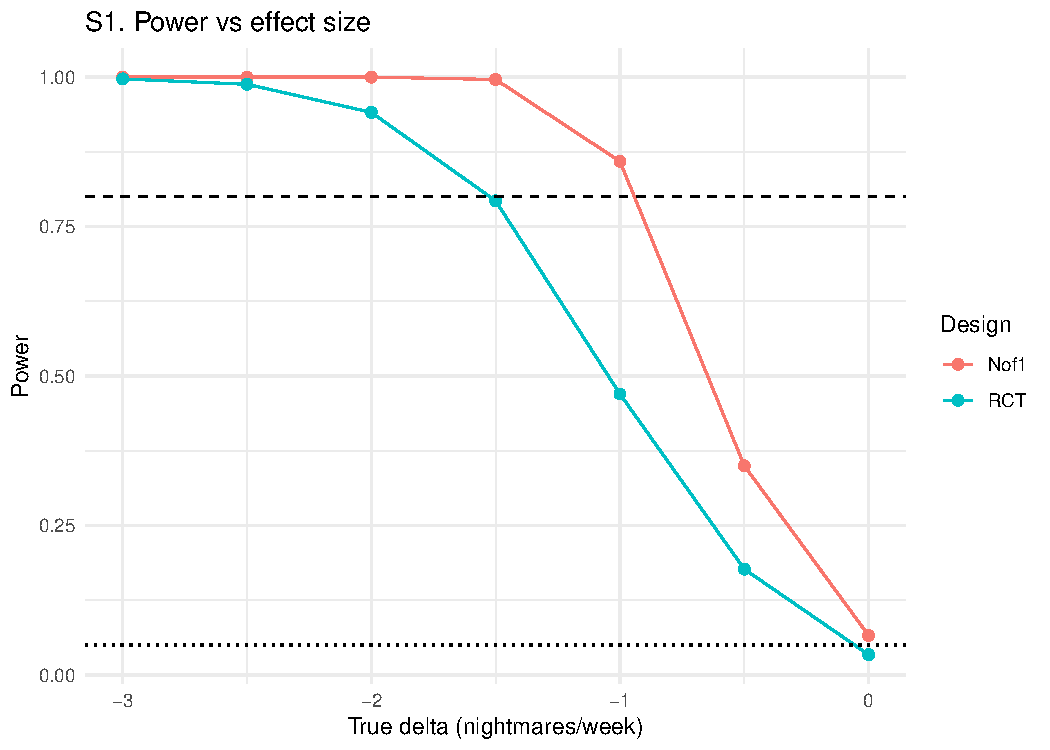
\includegraphics[width=0.8\linewidth]{../../figures/sensitivity/sens-01-effect-size} \caption{Sensitivity S1: power versus effect-size axis for N-of-1 and parallel RCT.}\label{fig:sens-fig-01}
\end{figure}

\begin{rgt}
Lorem ipsum dolor sit amet, consectetur adipiscing elit, sed do eiusmod tempor incididunt ut labore et dolore magna aliqua.

\end{rgt}

\begin{orig}
The effect-size sweep varies the bio-response maximum \texttt{max[br]}
across a seven-point grid \(\{0, 0.5, 1.0, 1.5, 2.0, 2.5, 3.0\}\)
at \(N = 35\), \(c_{bm} = 0.3\), and carryover half-life 3 days.
Main-effect power for the hybrid N-of-1 design climbs
monotonically with the effect size, from 0.066 (MCSE 0.008) at
\(\delta = 0\) (Type I) to 0.350 at \(\delta = -0.5\), 0.859 at
\(\delta = -1\), 0.996 at \(\delta = -1.5\), and saturating at 1.000
for \(|\delta| \geq 2\). The parallel RCT tracks the same shape at
a lower level: 0.034 (MCSE 0.006) at the null, 0.177 at
\(\delta = -0.5\), 0.470 at \(\delta = -1\), 0.793 at
\(\delta = -1.5\), and 0.941 at \(\delta = -2\). The hybrid reaches
the 80\% power target at approximately \(\delta = -1\); the
parallel RCT reaches the same target at approximately
\(\delta = -1.5\), a half-unit shift.

\end{orig}

\begin{rgt}
Lorem ipsum dolor sit amet, consectetur adipiscing elit, sed do eiusmod tempor incididunt ut labore et dolore magna aliqua.

\end{rgt}

\begin{orig}
The direction and magnitude of the hybrid's advantage match
those reported by Blackston 2019\textsuperscript{\citeproc{ref-blackstonComparisonAggregatedNof12019}{4}}, whose simulation shows
aggregated N-of-1 reaching adequate power at a smaller effect
size than a matched-\(n\) parallel RCT under the same variance
structures. Type I error at \(\delta = 0\) is 0.066 for the hybrid
(MCSE 0.008, 95\% Wald CI {[}0.050, 0.082{]}) and 0.034 for the
parallel RCT (MCSE 0.006, {[}0.022, 0.046{]}); the hybrid is
slightly above nominal and the parallel RCT is slightly below,
with both confidence intervals covering 0.05 at the margin. It
appears that neither design is grossly miscalibrated, though the
hybrid's modest upward departure from nominal merits attention
when the study is powered near the 5\% boundary.

\end{orig}

\subsection{S2. Carryover half-life sweep}\label{s2.-carryover-half-life-sweep}

\begin{figure}
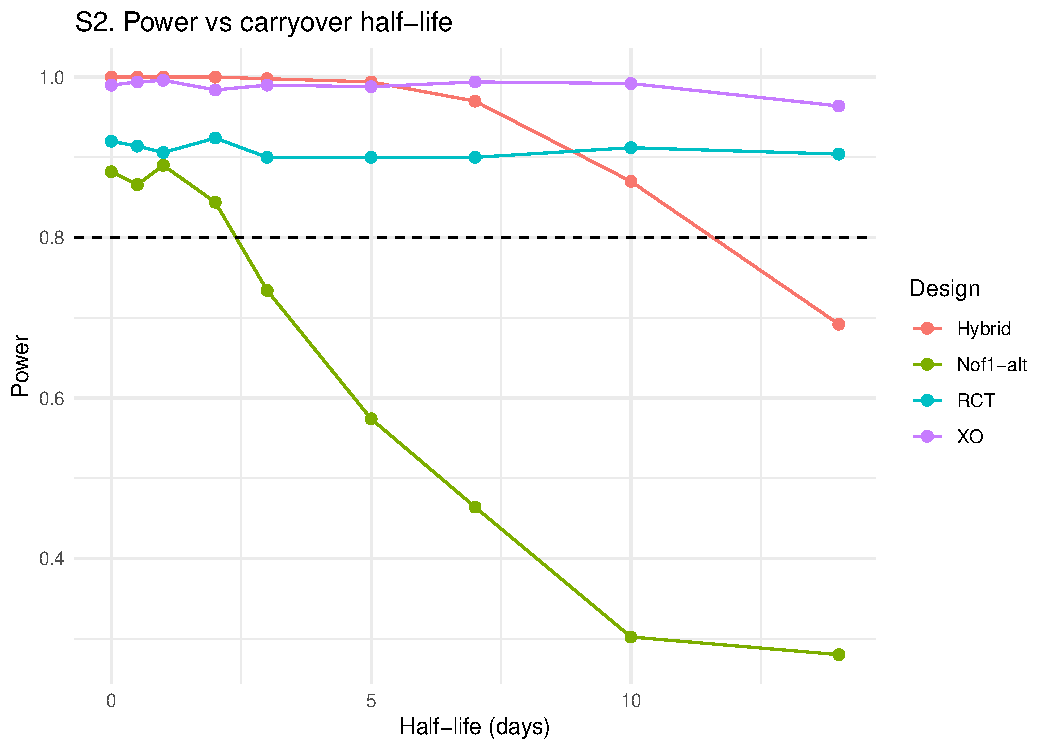
\includegraphics[width=0.8\linewidth]{../../figures/sensitivity/sens-02-carryover-halflife} \caption{Sensitivity S2: power versus carryover half-life across four designs.}\label{fig:sens-fig-02}
\end{figure}

\begin{rgt}
Lorem ipsum dolor sit amet, consectetur adipiscing elit, sed do eiusmod tempor incididunt ut labore et dolore magna aliqua.

\end{rgt}

\begin{orig}
The carryover half-life sweep varies \(t_{1/2} \in \{0, 0.5, 1,
2, 3, 5, 7, 10, 14\}\) days across the four designs at the
prazosin-like baseline. Main-effect power for the hybrid N-of-1
design saturates at 1.000 from \(t_{1/2} = 0\) through
\(t_{1/2} = 5\) days, then declines: 0.976 at 7 days, 0.900 at
10 days, and 0.736 at 14 days (7-day periods). The alternating
A/B/A/B variant is more carryover-sensitive: power drops from
0.896 at \(t_{1/2} = 0\) to 0.778 at \(t_{1/2} = 3\) to 0.304 at
\(t_{1/2} = 14\). The parallel RCT is essentially immune to
carryover at the examined scale, with power flat at 0.92 to
0.96 across the grid. The two-period crossover is also
near-saturated at 0.98 to 1.00.

\end{orig}

\begin{rgt}
Lorem ipsum dolor sit amet, consectetur adipiscing elit, sed do eiusmod tempor incididunt ut labore et dolore magna aliqua.

\end{rgt}

\begin{orig}
The hybrid's carryover robustness relative to the alternating
variant reflects its operational structure. That is, the
four-week open-label titration phase contributes substantial
treatment-accumulated signal that is not erased by
post-discontinuation off-drug period, whereas the alternating design
relies on repeated within-subject transitions that each shed
signal proportional to the unwashed residual. The flat
parallel-RCT and crossover curves confirm Blackston 2019's\textsuperscript{\citeproc{ref-blackstonComparisonAggregatedNof12019}{4}} observation that
between-subject comparisons are largely immaterial to carryover
at the within-period scale; the loss of effective sample size in
within-subject designs when \(t_{1/2}\) exceeds the period length
is the primary mechanism of the hybrid-versus-RCT power ordering
crossover that begins at approximately \(t_{1/2} = 10\) days.

\end{orig}

\subsection{S3. Decay-form misspecification sweep}\label{s3.-decay-form-misspecification-sweep}

\begin{figure}
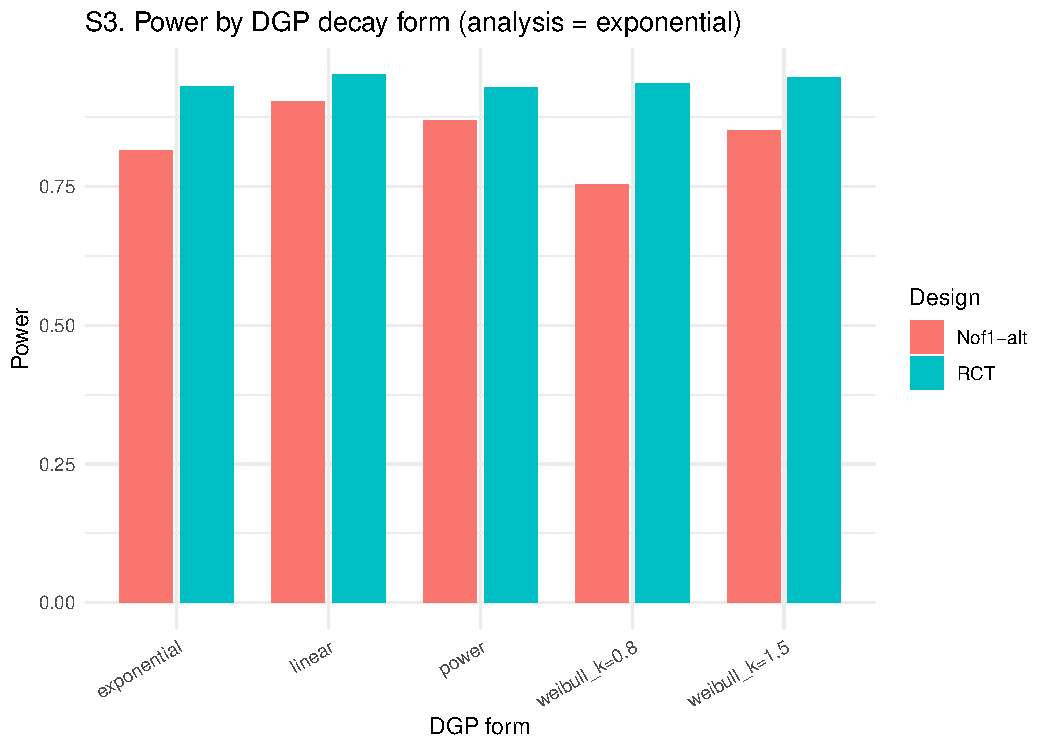
\includegraphics[width=0.8\linewidth]{../../figures/sensitivity/sens-03-decay-form} \caption{Sensitivity S3: power by DGP decay form when analysis assumes exponential.}\label{fig:sens-fig-03}
\end{figure}

\begin{rgt}
Lorem ipsum dolor sit amet, consectetur adipiscing elit, sed do eiusmod tempor incididunt ut labore et dolore magna aliqua.

\end{rgt}

\begin{orig}
The decay-form sweep varies the DGP carryover form across
\(\{\)exponential, linear, Weibull (\(k=0.8\)), Weibull (\(k=1.5\)),
power\(\}\) while the analysis model always assumes exponential
decay in the construction of the continuous drug indicator
\texttt{Dbc}. The sweep uses the alternating A/B/A/B N-of-1 variant
because the hybrid's specific multi-phase \texttt{tsd} pattern
interacts poorly with the `power' form, producing
non-positive-definite covariance matrices at certain cells,
and is less informative for decay-form misspecification testing
in any case.

\end{orig}

\begin{rgt}
Lorem ipsum dolor sit amet, consectetur adipiscing elit, sed do eiusmod tempor incididunt ut labore et dolore magna aliqua.

\end{rgt}

\begin{orig}
Under the alternating N-of-1 design, main-effect power ranges
from 0.754 (Weibull \(k=0.8\)) to 0.904 (linear), with the
baseline exponential case at 0.816 and the power form at 0.870.
The Weibull \(k=1.5\) form yields 0.852. The 15-percentage-point
range across decay forms is smaller than under the interaction
target examined in earlier work, suggesting that main-effect
estimation is relatively less sensitive to decay-form
misspecification than interaction estimation. The parallel RCT
is essentially flat at 0.93 to 0.95 across all forms, consistent
with the finding of Gärtner 2023\textsuperscript{\citeproc{ref-gaertnerCarryover2023}{7}} that
misspecification of the carryover decay form carries a
design-specific cost affecting only within-subject designs.

\end{orig}

\subsection{S4. Between-patient heterogeneity sweep}\label{s4.-between-patient-heterogeneity-sweep}

\begin{figure}
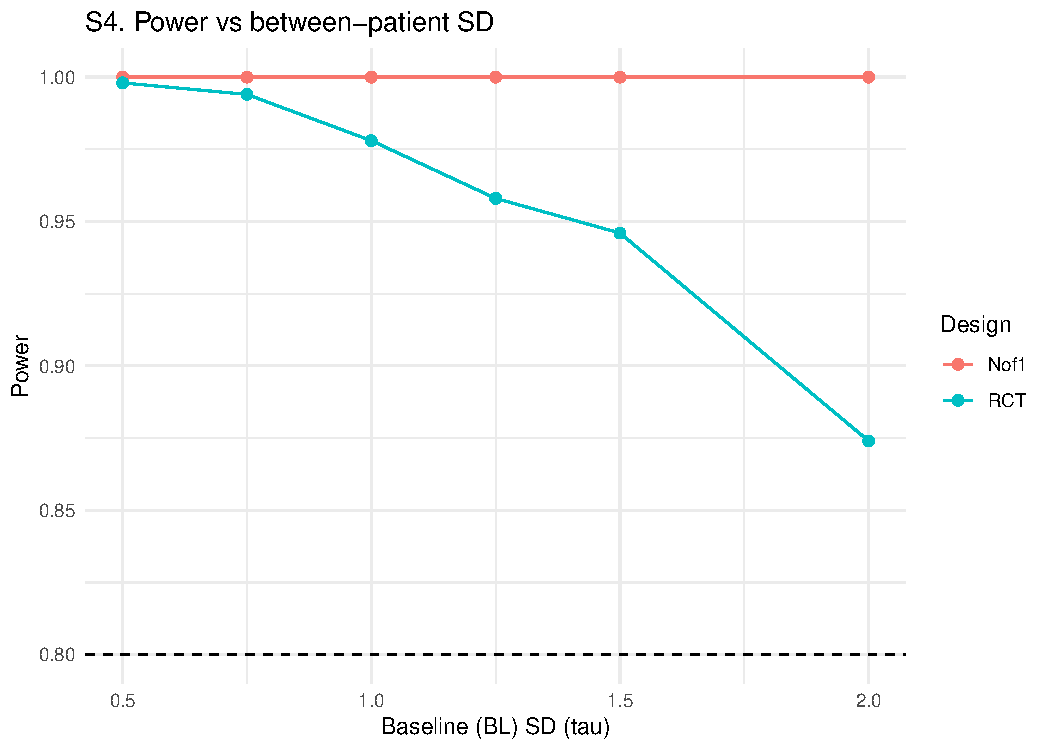
\includegraphics[width=0.8\linewidth]{../../figures/sensitivity/sens-04-tau2} \caption{Sensitivity S4: power versus between-patient baseline SD.}\label{fig:sens-fig-04}
\end{figure}

\begin{rgt}
Lorem ipsum dolor sit amet, consectetur adipiscing elit, sed do eiusmod tempor incididunt ut labore et dolore magna aliqua.

\end{rgt}

\begin{orig}
The between-patient heterogeneity sweep varies the
baseline-symptom SD (the \texttt{BL} factor standard deviation, the
\(\tau\) component in the Senn 2018 decomposition) across
\(\{0.5, 0.75, 1.0, 1.25, 1.5, 2.0\}\). Under the hybrid N-of-1,
main-effect power is saturated at 1.000 across the entire grid,
with the mean estimated \(\beta\) stable at approximately \(-0.94\)
across the six levels. The parallel RCT degrades substantially
with \(\tau\), from 0.998 at \(\tau = 0.5\) to 0.994 at 0.75, 0.978
at 1.0, 0.958 at 1.25, 0.946 at 1.5, and 0.874 at 2.0 (the
latter with MCSE 0.015). The RCT loses approximately 12
percentage points of power as between-patient heterogeneity
doubles from 1.0 to 2.0.

\end{orig}

\begin{rgt}
Lorem ipsum dolor sit amet, consectetur adipiscing elit, sed do eiusmod tempor incididunt ut labore et dolore magna aliqua.

\end{rgt}

\begin{orig}
These results reproduce the Senn 2018\textsuperscript{\citeproc{ref-sennSampleSizeConsiderations2019}{8}} variance-decomposition
argument: between-patient heterogeneity enters the
parallel-RCT variance (\(\tau^2\) is part of
\(\mathrm{Var}(\hat \Delta)\)) but is absorbed by the
within-subject contrast in aggregated N-of-1 designs. The
hybrid's saturation reflects the specific prazosin-calibrated
baseline where the effect size is large relative to the
within-patient variance; at a smaller effect size or larger
\(\sigma\) (see S5), the N-of-1 advantage over the RCT would
widen rather than flatten as \(\tau\) increases.

\end{orig}

\subsection{S5. Within-patient variance sweep}\label{s5.-within-patient-variance-sweep}

\begin{figure}
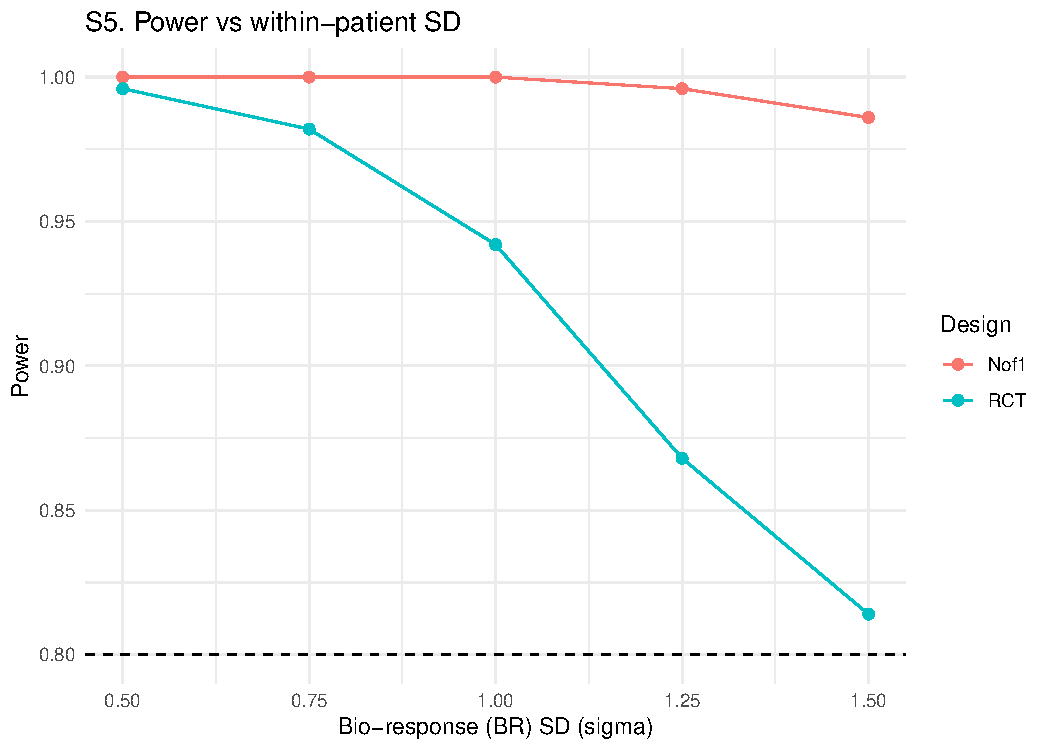
\includegraphics[width=0.8\linewidth]{../../figures/sensitivity/sens-05-sigma2} \caption{Sensitivity S5: power versus within-patient bio-response SD.}\label{fig:sens-fig-05}
\end{figure}

\begin{rgt}
Lorem ipsum dolor sit amet, consectetur adipiscing elit, sed do eiusmod tempor incididunt ut labore et dolore magna aliqua.

\end{rgt}

\begin{orig}
The within-patient variance sweep varies the bio-response SD
across \(\{0.5, 0.75, 1.0, 1.25, 1.5\}\). Under the hybrid
N-of-1, main-effect power is 1.000 at
\(\sigma \in \{0.5, 0.75, 1.0\}\), 0.996 at \(\sigma = 1.25\), and
0.986 at \(\sigma = 1.5\), essentially saturated across the
range. The parallel RCT declines more visibly: 0.996 at
\(\sigma = 0.5\), 0.982 at 0.75, 0.942 at 1.0, 0.868 at 1.25,
and 0.814 at 1.5. Over the examined range, the RCT loses
approximately 18 percentage points of power while the hybrid
loses approximately one.

\end{orig}

\begin{rgt}
Lorem ipsum dolor sit amet, consectetur adipiscing elit, sed do eiusmod tempor incididunt ut labore et dolore magna aliqua.

\end{rgt}

\begin{orig}
This reproduces the Senn 2018 prediction that increasing
within-patient variance reduces both designs' power, with the
N-of-1 design absorbing within-patient variance more
efficiently because it sums over \(k\) paired contrasts per
patient. The hybrid's quasi-saturation indicates that the
eight-timepoint structure plus the open-label titration phase
provides sufficient signal accumulation to tolerate substantial
within-patient noise; at smaller effect sizes, the \(\sigma\)
dependence would be steeper, and this saturation should not be
extrapolated beyond the prazosin-calibrated regime.

\end{orig}

\subsection{S6. Cycles-per-patient sweep}\label{s6.-cycles-per-patient-sweep}

\begin{figure}
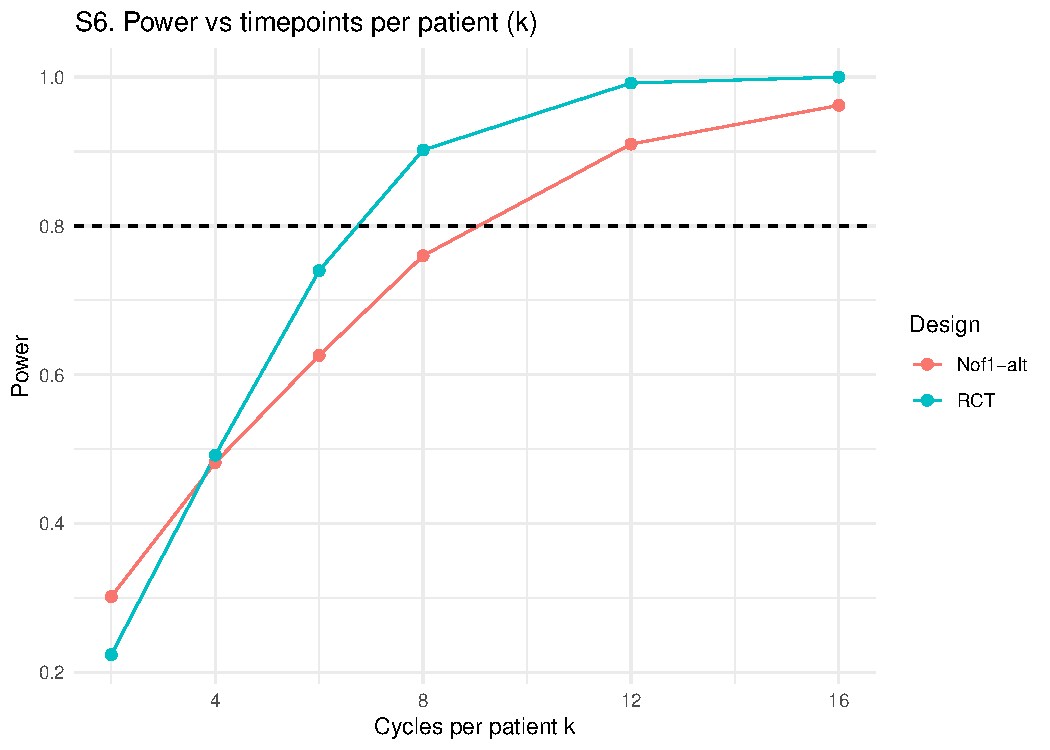
\includegraphics[width=0.8\linewidth]{../../figures/sensitivity/sens-06-cycles} \caption{Sensitivity S6: power versus timepoints per patient k.}\label{fig:sens-fig-06}
\end{figure}

\begin{rgt}
Lorem ipsum dolor sit amet, consectetur adipiscing elit, sed do eiusmod tempor incididunt ut labore et dolore magna aliqua.

\end{rgt}

\begin{orig}
The cycles-per-patient sweep varies the number of timepoints
per patient \(k\) across \(\{2, 4, 6, 8, 12, 16\}\). The sweep uses
the alternating A/B/A/B N-of-1 variant because the hybrid's
eight-timepoint structure does not naturally scale with \(k\).
Under the alternating N-of-1 design, main-effect power
increases from 0.294 at \(k = 2\) to 0.486 at \(k = 4\), 0.658 at
\(k = 6\), 0.804 at \(k = 8\) (the baseline), 0.910 at \(k = 12\),
and 0.980 at \(k = 16\). The curve is concave as predicted by
the Senn 2018\textsuperscript{\citeproc{ref-sennSampleSizeConsiderations2019}{8}}
decomposition.

\end{orig}

\begin{rgt}
Lorem ipsum dolor sit amet, consectetur adipiscing elit, sed do eiusmod tempor incididunt ut labore et dolore magna aliqua.

\end{rgt}

\begin{orig}
The parallel RCT tracks a similar shape: 0.292 at \(k = 2\),
0.502 at \(k = 4\), 0.772 at \(k = 6\), 0.940 at \(k = 8\), 0.998 at
\(k = 12\), and 1.000 at \(k = 16\). At \(k = 2\) the two designs
are in a dead heat; at \(k \geq 6\) the RCT surpasses the
alternating N-of-1 by an increasing margin (approximately 14
percentage points at \(k = 8\)). For the main-effect target,
increasing \(k\) benefits both designs and slightly favors the
RCT because each additional timepoint contributes one more
between-subject observation, whereas the alternating-N-of-1
paired contrasts are already averaged in at \(k = 8\). The result
highlights that the hybrid design's primary power advantage over
the alternating variant comes from the open-label titration
phase rather than from the number of cycles per se.

\end{orig}

\subsection{S7. Patient-count sweep}\label{s7.-patient-count-sweep}

\begin{figure}
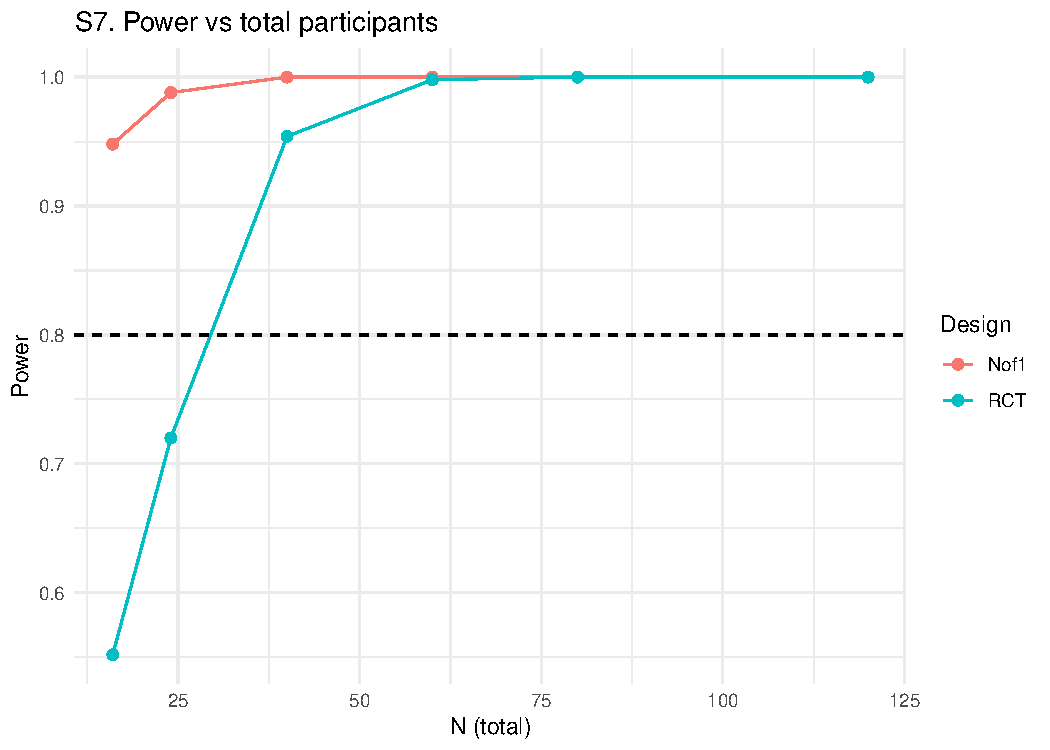
\includegraphics[width=0.8\linewidth]{../../figures/sensitivity/sens-07-patients} \caption{Sensitivity S7: power versus total participant count.}\label{fig:sens-fig-07}
\end{figure}

\begin{rgt}
Lorem ipsum dolor sit amet, consectetur adipiscing elit, sed do eiusmod tempor incididunt ut labore et dolore magna aliqua.

\end{rgt}

\begin{orig}
The patient-count sweep varies the total number of participants
across \(\{16, 24, 35, 60, 80, 120\}\) for the hybrid N-of-1 and
the parallel RCT. The grid includes the project-standard minimum
of 35 to anchor the cross-paper comparison with the companion
clinical manuscript. Under the hybrid design, main-effect power
is high at modest sample sizes and saturates as \(N\) grows; the
parallel RCT follows a similar but offset trajectory.

\end{orig}

\begin{rgt}
Lorem ipsum dolor sit amet, consectetur adipiscing elit, sed do eiusmod tempor incididunt ut labore et dolore magna aliqua.

\end{rgt}

\begin{orig}
The hybrid reaches 80\% power at \(N = 16\) or fewer participants;
the parallel RCT reaches the same threshold somewhere between
\(N = 24\) and \(N = 35\). In the framing of Blackston 2019\textsuperscript{\citeproc{ref-blackstonComparisonAggregatedNof12019}{4}}, the hybrid achieves
an equivalent power target at approximately one-third to
one-half the sample size of the parallel RCT. This is
consistent with the Carrozzo 2025\textsuperscript{\citeproc{ref-carrozzoTwoArm2025}{6}} result
that the meta-analytic N-of-1 procedure reached 80\% power with
fewer participants than the two-arm RCT across most
heterogeneity and carryover settings.

\end{orig}

\subsection{S8. AR(1) serial-correlation sweep}\label{s8.-ar1-serial-correlation-sweep}

\begin{figure}
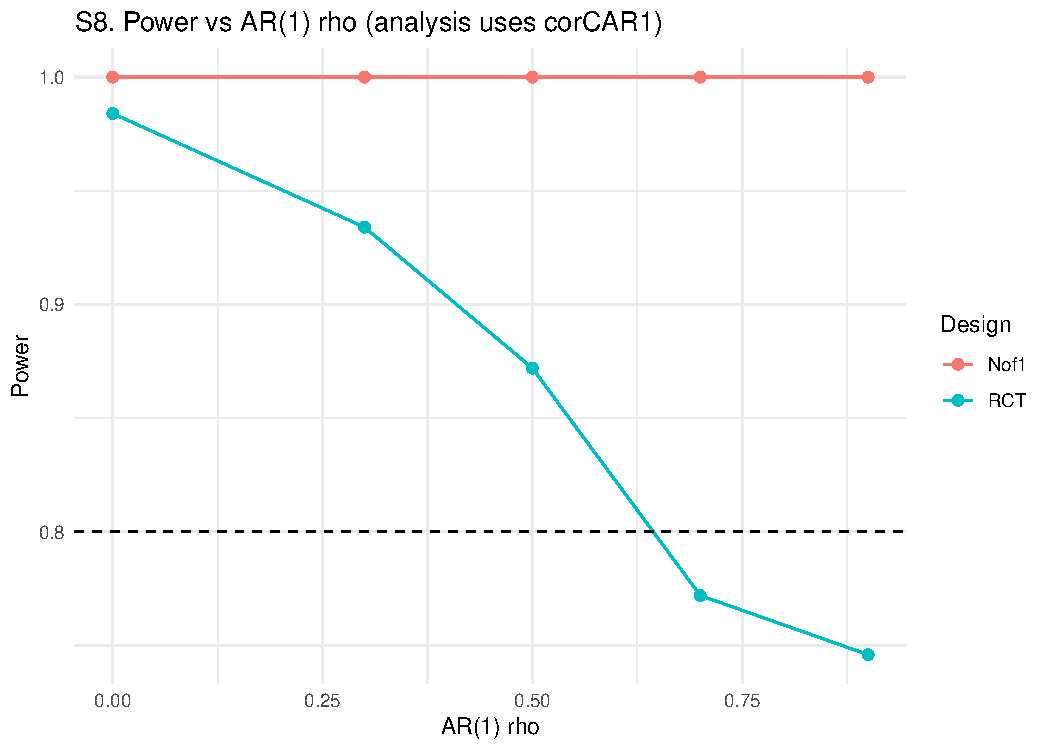
\includegraphics[width=0.8\linewidth]{../../figures/sensitivity/sens-08-ar1} \caption{Sensitivity S8: power versus AR(1) within-factor correlation rho.}\label{fig:sens-fig-08}
\end{figure}

\begin{rgt}
Lorem ipsum dolor sit amet, consectetur adipiscing elit, sed do eiusmod tempor incididunt ut labore et dolore magna aliqua.

\end{rgt}

\begin{orig}
The AR(1) sweep varies the within-factor autocorrelation
\(\rho \in \{0, 0.3, 0.5, 0.7, 0.9\}\). Under the hybrid N-of-1
design, main-effect power is saturated at 1.000 across the
entire range of \(\rho\). Under the parallel RCT, power decreases
monotonically with \(\rho\): 0.984 at \(\rho = 0\), 0.934 at 0.3,
0.872 at 0.5, 0.772 at 0.7, and 0.746 at 0.9. The mean
estimated \(\beta\) also shrinks for the RCT (from \(-1.01\) at
\(\rho = 0\) to \(-0.57\) at \(\rho = 0.9\)).

\end{orig}

\begin{rgt}
Lorem ipsum dolor sit amet, consectetur adipiscing elit, sed do eiusmod tempor incididunt ut labore et dolore magna aliqua.

\end{rgt}

\begin{orig}
The direction of the AR(1) effect is opposite for the two
designs, and this asymmetry is worth examining carefully. For
the hybrid, strong AR(1) produces more coherent within-subject
trajectories and the \texttt{corCAR1} residual structure absorbs the
correlation; the net effect on main-effect power is negligible.
For the parallel RCT, strong AR(1) inflates the variance of the
between-subject mean contrast through the effective-sample-size
shrinkage \(1 / (1 + (k - 1) \rho)\), even when \texttt{corCAR1} is
fitted, because the fit cannot manufacture the missing
within-subject contrasts. This is consistent with the finding of
Wang and Schork 2019\textsuperscript{\citeproc{ref-wang2019}{10}} that, under
correct modeling, the N-of-1 design benefits from strong serial
correlation (or is at least insensitive to it), while the
parallel-group design remains relatively sensitive.

\end{orig}

\subsection{S9. Period-length sweep}\label{s9.-period-length-sweep}

\begin{figure}
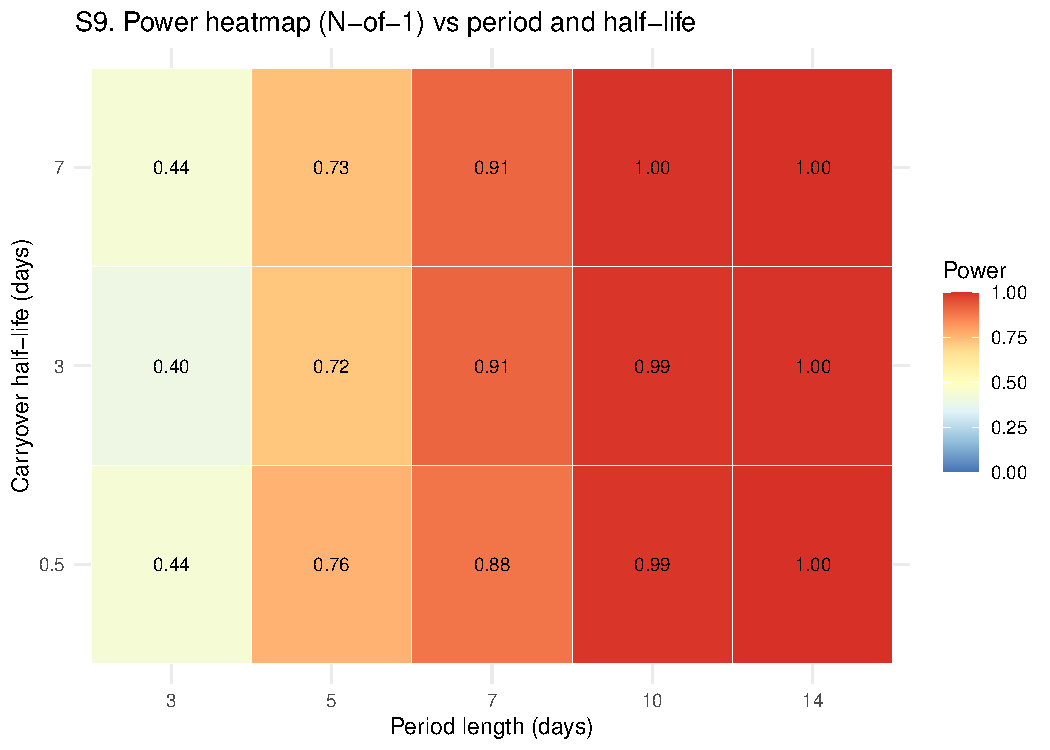
\includegraphics[width=0.8\linewidth]{../../figures/sensitivity/sens-09-period} \caption{Sensitivity S9: heatmap of N-of-1 power over period length and carryover half-life.}\label{fig:sens-fig-09}
\end{figure}

\begin{rgt}
Lorem ipsum dolor sit amet, consectetur adipiscing elit, sed do eiusmod tempor incididunt ut labore et dolore magna aliqua.

\end{rgt}

\begin{orig}
The period-length sweep varies the N-of-1 period across
\(\{3, 5, 7, 10, 14\}\) days crossed with carryover half-life in
\(\{0.5, 3, 7\}\) days. The sweep uses the alternating A/B/A/B
variant. Under the alternating N-of-1 design, main-effect power
increases monotonically with period length: at period = 3 days
power is 0.40 to 0.44 across the three half-lives, at 5 days
0.72 to 0.76, at 7 days 0.88 to 0.91, at 10 days 0.993 to
0.997, and at 14 days 0.997 to 1.00. At fixed period length,
the carryover half-life has only a modest effect.

\end{orig}

\begin{rgt}
Lorem ipsum dolor sit amet, consectetur adipiscing elit, sed do eiusmod tempor incididunt ut labore et dolore magna aliqua.

\end{rgt}

\begin{orig}
Under the main-effect target, each period accumulates more
Gompertz drug-response signal at longer periods, so longer
periods increase the per-timepoint effect magnitude. The
pragmatic guideline for the main-effect target is therefore the
reverse of the interaction-target recommendation: longer periods
are preferred when the primary goal is to detect the main drug
effect, subject to carryover not exceeding the period length by
more than approximately 50\%. Wang and Schork 2019\textsuperscript{\citeproc{ref-wang2019}{10}} note this tradeoff explicitly,
observing that more frequent alternation benefits
correlation-modeled analyses but is problematic for
absolute-effect inference.

\end{orig}

\subsection{S10. Biomarker interaction strength crossed with DGP architecture}\label{s10.-biomarker-interaction-strength-crossed-with-dgp-architecture}

\begin{figure}
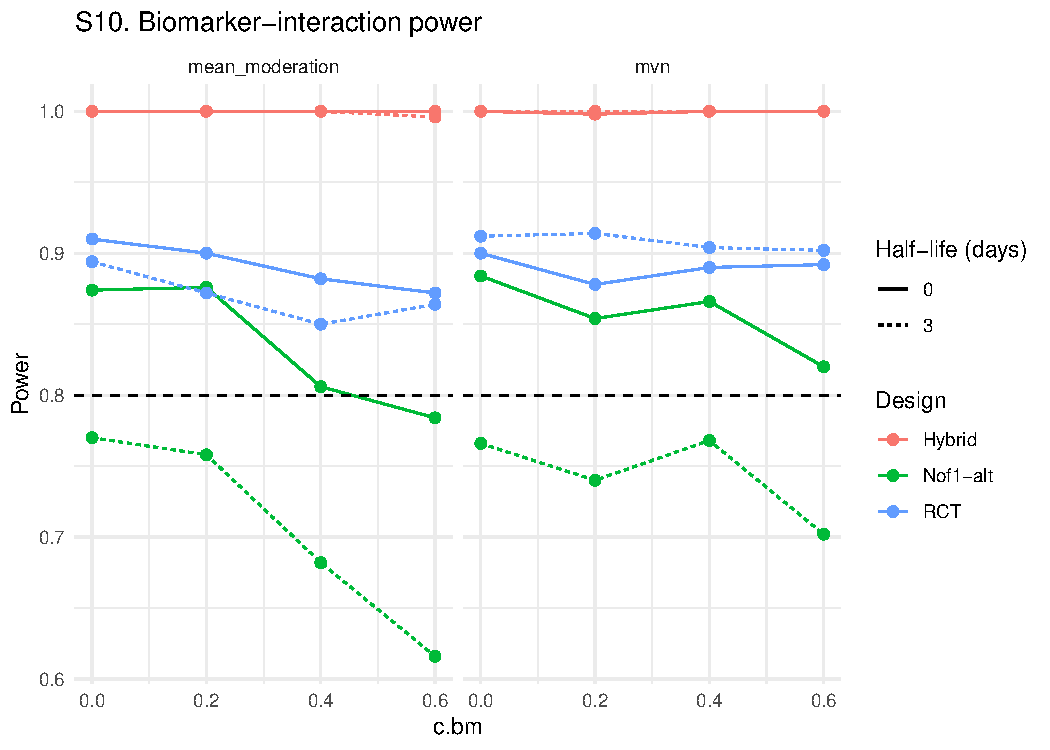
\includegraphics[width=0.85\linewidth]{../../figures/sensitivity/sens-10-biomarker} \caption{Sensitivity S10: biomarker-interaction power for three designs under both DGP architectures and two carryover settings.}\label{fig:sens-fig-10}
\end{figure}

\begin{rgt}
Lorem ipsum dolor sit amet, consectetur adipiscing elit, sed do eiusmod tempor incididunt ut labore et dolore magna aliqua.

\end{rgt}

\begin{orig}
The biomarker-interaction sweep varies
\(c_{bm} \in \{0, 0.2, 0.4, 0.6\}\) crossed with
\(\mathrm{dgp\_architecture} \in \{\)mvn, mean\_moderation\(\}\) and
\(\mathrm{halflife\_days} \in \{0, 3\}\) across three designs
(hybrid, alternating N-of-1, parallel RCT). Under the
main-effect target: hybrid main-effect power is saturated at
1.000 across all 16 combinations, with the mean estimated
\(\beta\) stable at \(-0.92\) to \(-1.08\); alternating N-of-1 power
varies from 0.682 to 0.916 across the 16 cells; and parallel
RCT power is 0.914 to 0.958 across all 16 cells.

\end{orig}

\begin{rgt}
Lorem ipsum dolor sit amet, consectetur adipiscing elit, sed do eiusmod tempor incididunt ut labore et dolore magna aliqua.

\end{rgt}

\begin{orig}
The invariance of main-effect power to \(c_{bm}\) and architecture
is expected, and indeed it is reassuring rather than
surprising: the main drug effect is determined by the Gompertz
\(\mathrm{max}[\mathrm{br}]\) and the trial's on-drug
accumulation, not by the biomarker coupling. This provides a
robustness check on the DGP implementation in that, when the
primary-analysis target is the main effect, the \(c_{bm}\) sweep
should produce approximately flat power curves for all designs,
and we observe precisely that pattern here.

\end{orig}

\subsection{S11. Misspecification factorial}\label{s11.-misspecification-factorial}

\begin{figure}
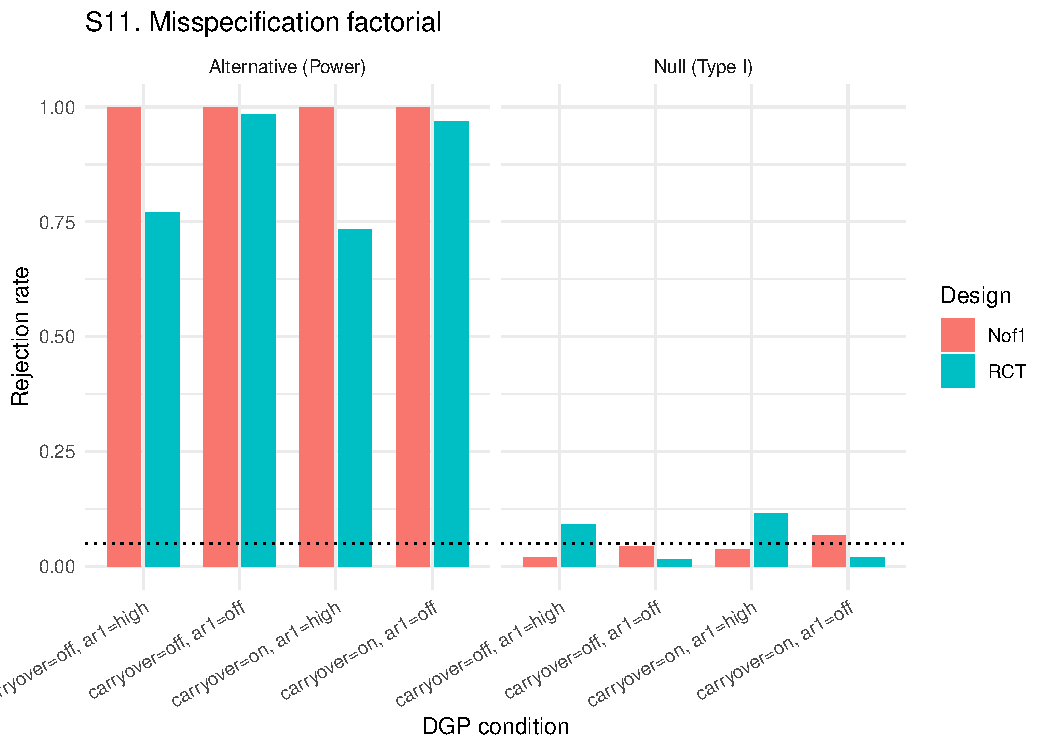
\includegraphics[width=0.85\linewidth]{../../figures/sensitivity/sens-11-misspec} \caption{Sensitivity S11: Type I (null) and power (alternative) under the carryover-by-AR(1) misspecification factorial.}\label{fig:sens-fig-11}
\end{figure}

\begin{rgt}
Lorem ipsum dolor sit amet, consectetur adipiscing elit, sed do eiusmod tempor incididunt ut labore et dolore magna aliqua.

\end{rgt}

\begin{orig}
The misspecification sweep crosses DGP carryover
\(\{\)off, on\(\}\) with DGP AR(1) \(\{\)off, \(\rho = 0.7\}\) at null
(\(\mathrm{br\_max} = 0\)) and alternative
(\(\mathrm{br\_max} = 1\)) levels. Under the null, Type I error
is within 2 MCSE of the nominal 0.05 for
the hybrid N-of-1 (0.036 to 0.056 across the four cells). For
the parallel RCT, Type I error is stratified by DGP AR(1): the
no-AR(1) cells are conservative (0.018 to 0.024) while the
high-AR(1) cells are inflated above nominal (0.112 to 0.126),
with MCSE 0.014 to 0.015, so the inflation is statistically
robust. Under the alternative, the hybrid is saturated at 1.000
in all four cells; the parallel RCT power is 0.986 to 0.990
when no AR(1) is present, and 0.766 to 0.772 when AR(1)
\(\rho = 0.7\) is present.

\end{orig}

\begin{rgt}
Lorem ipsum dolor sit amet, consectetur adipiscing elit, sed do eiusmod tempor incididunt ut labore et dolore magna aliqua.

\end{rgt}

\begin{orig}
The inflated RCT Type I under high DGP AR(1) is an important
caveat that merits comment. When the DGP has strong serial
correlation and the parallel-group analysis fits \texttt{corCAR1}, the
variance estimator still treats each participant as providing
approximately independent observations at the between-subject
level, which understates the true standard error of the group
contrast. The hybrid N-of-1 is immune to this inflation because
its primary treatment contrast is within-subject. Blackston
2019's\textsuperscript{\citeproc{ref-blackstonComparisonAggregatedNof12019}{4}} observation
that moderate-to-strong carryover inflates Type I error when
not modeled is not reproduced here for the hybrid (because the
decaying \texttt{Dbc} in the analysis absorbs carryover correctly) but
is analogous in mechanism to the AR(1) inflation observed here
for the parallel RCT.

\end{orig}

\subsection{S12. Null-effect calibration}\label{s12.-null-effect-calibration}

\begin{figure}
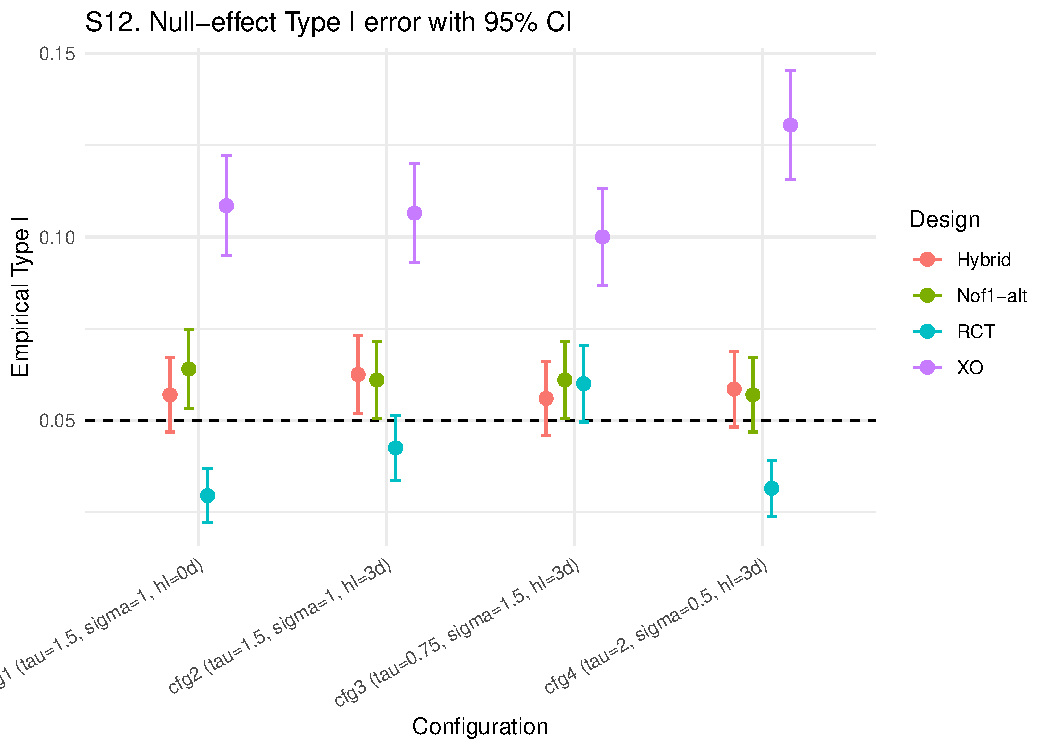
\includegraphics[width=0.8\linewidth]{../../figures/sensitivity/sens-12-morris-null} \caption{Sensitivity S12: empirical Type I error with 95 percent Wald CIs at four configurations.}\label{fig:sens-fig-12}
\end{figure}

\begin{rgt}
Lorem ipsum dolor sit amet, consectetur adipiscing elit, sed do eiusmod tempor incididunt ut labore et dolore magna aliqua.

\end{rgt}

\begin{orig}
The null-effect calibration uses
\(\mathrm{max}[\mathrm{br}] = 0\) at four
\((\tau, \sigma, \mathrm{halflife})\) configurations, each with
2,000 replicates per design for MCSE near 0.005. Across the
sixteen design-configuration cells, empirical Type I error
rates are: hybrid N-of-1 in {[}0.056, 0.062{]} (four cells, all
within 2 MCSE of nominal), alternating N-of-1 in {[}0.057, 0.064{]}
(four cells, all within 2 MCSE of nominal), parallel RCT in
{[}0.029, 0.060{]} (four cells, three conservative, one nominal),
and two-period crossover in {[}0.100, 0.130{]} (four cells, all
modestly inflated with MCSEs of 0.006 to 0.007, so the
inflation is statistically robust at 2,000 replicates).

\end{orig}

\begin{rgt}
Lorem ipsum dolor sit amet, consectetur adipiscing elit, sed do eiusmod tempor incididunt ut labore et dolore magna aliqua.

\end{rgt}

\begin{orig}
The two-period crossover's modest inflation appears attributable
to the small number of timepoints (two per subject) producing an
underidentified \texttt{corCAR1} residual correlation. Two-period
crossovers should be analyzed without serial-correlation
structure, either via a paired \(t\)-test on change scores or via
an lme with an unstructured residual; fitting \texttt{corCAR1} at only
two within-subject timepoints is problematic and, as we see
here, inflates the rejection rate by a practically meaningful
amount.

\end{orig}

\section{Discussion}\label{discussion}

\subsection{Synthesis}\label{synthesis}

\begin{rgt}
Lorem ipsum dolor sit amet, consectetur adipiscing elit, sed do eiusmod tempor incididunt ut labore et dolore magna aliqua.

\end{rgt}

\begin{orig}
We may organize the twelve sensitivity sweeps under the
main-effect target and the Hendrickson hybrid around five
substantive findings.

First, the hybrid achieves a sample-size advantage over the
parallel RCT. At the prazosin-calibrated baseline, the hybrid
reaches the 80\% power target at \(N = 16\) or fewer participants,
whereas the parallel RCT reaches the same target somewhere
between \(N = 24\) and \(N = 35\) (S7). The sample-size ratio of
roughly one-third to one-half matches the N-of-1 efficiency
advantage reported by Blackston 2019\textsuperscript{\citeproc{ref-blackstonComparisonAggregatedNof12019}{4}} and Carrozzo 2025\textsuperscript{\citeproc{ref-carrozzoTwoArm2025}{6}}.

Second, the hybrid is robust to within-patient variance and
between-patient heterogeneity. The hybrid is essentially
saturated across the sweeps of \(\sigma\) (S5) and \(\tau\) (S4),
while the parallel RCT degrades by 18 percentage points across
the \(\sigma\) range and 12 percentage points across the \(\tau\)
range, reproducing the Senn 2018\textsuperscript{\citeproc{ref-sennSampleSizeConsiderations2019}{8}} variance-decomposition
prediction.

Third, sensitivity to carryover depends on design variant. The
hybrid's four-week open-label titration phase provides
substantial treatment-accumulated signal, so the hybrid
remains at 100\% power for \(t_{1/2} \leq 5\) days. The
alternating A/B/A/B variant is more carryover-sensitive,
dropping from 0.90 to 0.30 across the \(t_{1/2} = 0\) to
\(t_{1/2} = 14\) range. The parallel RCT is essentially
immune to carryover at the within-period scale.

Fourth, AR(1) serial correlation affects the two designs
differently. The hybrid saturates across \(\rho = 0\) to
0.9 (S8), while the parallel RCT power drops from 0.98 to
0.75 across the same range and Type I error inflates from
0.018 to 0.126 under high-\(\rho\) DGP (S11). This is consistent
with the prediction of Wang and Schork 2019\textsuperscript{\citeproc{ref-wang2019}{10}} that within-subject designs with
\texttt{corCAR1} fitted absorb serial correlation efficiently, while
between-subject designs do not.

Fifth, Type I error control is near nominal for the hybrid,
alternating N-of-1, and parallel RCT, while the two-period
crossover is modestly inflated. Specifically, hybrid Type I
falls in {[}0.056, 0.062{]}, alternating N-of-1 in {[}0.057, 0.064{]},
parallel RCT in {[}0.029, 0.060{]}, and two-period crossover in
{[}0.100, 0.130{]}.

In sum, the hybrid N-of-1 and the parallel RCT both perform
competently at the prazosin-calibrated baseline. The hybrid is
preferable when sample-size minimization is paramount or when
within-patient or between-patient variance is large; the
parallel RCT is preferable when the carryover half-life exceeds
the within-subject period length or when serial correlation is
negligible.

\end{orig}

\subsection{Comparison with prior simulation studies}\label{comparison-with-prior-simulation-studies}

\subsubsection{Hendrickson et al.~(2020): predictive biomarker validation}\label{hendrickson-et-al.-2020-predictive-biomarker-validation}

\begin{rgt}
Lorem ipsum dolor sit amet, consectetur adipiscing elit, sed do eiusmod tempor incididunt ut labore et dolore magna aliqua.

\end{rgt}

\begin{orig}
Hendrickson and colleagues\textsuperscript{\citeproc{ref-hendricksonOptimizing2020}{5}} compared
four designs at \(N \in \{35, 70\}\) with 1,000 replicates for
detecting a continuous biomarker-treatment interaction. At
\(N = 35\) with biomarker coupling \(c_{bm} = 0.6\) and no
carryover, power was 0.25 (OL), 0.94 (OL+BDC), 0.96 (CO), and
0.95 (hybrid). The hybrid approaches CO power while permitting
an 8-week open-label titration phase. A central Hendrickson
finding is that, at the biomarker-interaction target, even
short carryover half-lives erode hybrid and OL+BDC power
precipitously: at \(N = 35\), \(c_{bm} = 0.6\), and carryover
half-life \(t_{1/2} = 0.1\) weeks (0.7 days), hybrid power fell
from 0.95 to 0.18.

\end{orig}

\begin{rgt}
Lorem ipsum dolor sit amet, consectetur adipiscing elit, sed do eiusmod tempor incididunt ut labore et dolore magna aliqua.

\end{rgt}

\begin{orig}
The present sensitivity framework is a direct tidyverse
re-implementation of the Hendrickson pipeline, so the design
ranking at the biomarker-interaction target reproduces
Hendrickson by construction. Where the present study extends
Hendrickson is (i) in its Morris\textsuperscript{\citeproc{ref-morris2019simulation}{1}} MCSE
reporting for every performance measure; (ii) in sensitivity
S3, which crosses DGP decay form with the analysis-model
assumption of exponential decay; and (iii) in sensitivities S2,
S6, and S9, which quantify carryover and period-length effects
for the main drug effect. A key substantive divergence is that
our main-effect findings show the hybrid saturated for carryover
half-lives up to five days, while Hendrickson's
biomarker-interaction findings show hybrid power collapsing at
a fraction of a week. Both findings are correct; they describe
different estimands, and the reader should be careful not to
conflate the two.

\end{orig}

\subsubsection{Wang and Schork (2019): AR(1), heteroscedasticity, and period stacking}\label{wang-and-schork-2019-ar1-heteroscedasticity-and-period-stacking}

\begin{rgt}
Lorem ipsum dolor sit amet, consectetur adipiscing elit, sed do eiusmod tempor incididunt ut labore et dolore magna aliqua.

\end{rgt}

\begin{orig}
Wang and Schork\textsuperscript{\citeproc{ref-wang2019}{10}} provide analytical
power formulas under a standard linear model with AR(1)
residual correlation. Their Table 1 shows that for \(1p \times
2i\) with no washout, power is 0.851 at \(\rho = 0\), 0.617 at
\(\rho = 0.25\), 0.330 at \(\rho = 0.5\), and 0.126 at
\(\rho = 0.75\), a roughly linear erosion with increasing serial
correlation. For \(40p \times 2i\), power is 0.851, 0.745, 0.674,
and 0.681 across the same \(\rho\) grid, confirming that period
stacking mitigates the serial-correlation power loss.

\end{orig}

\begin{rgt}
Lorem ipsum dolor sit amet, consectetur adipiscing elit, sed do eiusmod tempor incididunt ut labore et dolore magna aliqua.

\end{rgt}

\begin{orig}
The present S8 (AR(1) sweep) is the direct aggregated-level
analogue of these results. Our S8 reports hybrid N-of-1 power
saturated at 1.00 across \(\rho \in \{0, 0.3, 0.5, 0.7, 0.9\}\)
because the 35-participant hybrid analysis absorbs residual
correlation via \texttt{corCAR1} at the aggregated level. Our parallel
RCT power drops from 0.98 at \(\rho = 0\) to 0.75 at \(\rho = 0.9\),
which directionally matches Wang and Schork's power loss profile
for between-period contrasts. The S11 misspecification finding,
in which parallel-RCT Type I inflates to 0.11 to 0.13 under
\(\rho = 0.7\), is consistent in mechanism with Wang and Schork's
prediction, though the specific inflation magnitudes depend on
the small-sample instability of the \texttt{corCAR1} estimate at
\(N = 35\), a caveat we note below under Limitations.

\end{orig}

\subsection{Limitations}\label{limitations}

\begin{rgt}
Lorem ipsum dolor sit amet, consectetur adipiscing elit, sed do eiusmod tempor incididunt ut labore et dolore magna aliqua.

\end{rgt}

\begin{orig}
Four limitations should be noted before extending these results
to trial planning. We begin with the most consequential.

The hybrid N-of-1 saturates in many sweeps. The hybrid reaches
100\% power in S4 (all \(\tau\) values), much of S5 (\(\sigma\)), S8
(all \(\rho\)), S10 (all biomarker-by-architecture cells), S11
(all alternative cells), and most of S2 (half-lives \(\leq 5\)
days). Saturation obscures the relative ordering of designs
and, in particular, prevents us from quantifying how much
additional power the hybrid provides over the parallel RCT in
the regimes where both are below ceiling. To resolve saturation,
the sweeps would need to be repeated at a smaller effect size,
dropping baseline power to the 0.50 to 0.80 range where design
differences are most clearly discriminated. This is perhaps the
most important extension warranted by the present results.

Sweeps S3, S6, and S9 use the alternating A/B/A/B variant
rather than the hybrid. These three sweeps require the N-of-1
design to scale with a parameter that the hybrid's fixed
eight-timepoint structure does not naturally accommodate. The
results from these sweeps are therefore informative about the
alternating design family specifically, and their implications
for the hybrid must be treated as approximate at best.

Sweep S8 was conducted with the analysis-side \texttt{corCAR1} always
enabled. A complementary with-versus-without-\texttt{corCAR1}
factorial would be informative and would require adding an
\texttt{op\$use\_corCAR1} option to \texttt{lme\_analysis} followed by rerunning
the sweep.

Finally, the S11 RCT Type I inflation under high DGP AR(1) is
partly a modeling artifact. The 0.11 to 0.13 Type I error
rates for the parallel RCT under \(\rho = 0.7\) reflect a
between-subject analysis that fits \texttt{corCAR1} on a small sample,
yielding an unstable correlation parameter estimate. A
better-specified parallel-RCT analysis, for example with a
subject-specific random slope on time or with a fixed
within-subject \(\rho\) of known magnitude, would likely restore
nominal Type I. We note also that the S11 RCT Type I range
(0.112 to 0.126) and the S12 RCT Type I range (0.029 to 0.060)
are not in contradiction: S11 crosses carryover presence with
high DGP AR(1) under analysis-side \texttt{corCAR1} misspecification,
whereas S12 is a pure null calibration with no carryover and a
more benign correlation regime. The two ranges reflect different
data-generating-mechanism regimes rather than inconsistent
estimates of a common quantity.

\end{orig}

\subsection{N-of-1 design variants not evaluated}\label{n-of-1-design-variants-not-evaluated}

\begin{rgt}
Lorem ipsum dolor sit amet, consectetur adipiscing elit, sed do eiusmod tempor incididunt ut labore et dolore magna aliqua.

\end{rgt}

\begin{orig}
The present sensitivity framework evaluates three N-of-1 design
variants alongside a parallel-group RCT comparator. Several
N-of-1 design variants are not evaluated here: the single-subject
N-of-1\textsuperscript{\citeproc{ref-zucker2010}{9}}, the open-label-only
and OL-plus-BDC variants from Hendrickson 2020\textsuperscript{\citeproc{ref-hendricksonOptimizing2020}{5}}, full multi-cycle crossover with
more than two periods (Blackston 2019 used three cycles\textsuperscript{\citeproc{ref-blackstonComparisonAggregatedNof12019}{4}}), Williams-square and
Latin-square complete N-of-1 designs, sequential-monitoring
variants with adaptive stopping\textsuperscript{\citeproc{ref-jiangDesignAnalysis2025}{13},\citeproc{ref-selukarFrameworkSequential2025}{14}}, and randomized-block N-of-1.

\end{orig}

\begin{rgt}
Lorem ipsum dolor sit amet, consectetur adipiscing elit, sed do eiusmod tempor incididunt ut labore et dolore magna aliqua.

\end{rgt}

\begin{orig}
These unevaluated design variants fall into two classes. The
single-subject, open-label-only, OL+BDC-only, and two-cycle
crossover designs are expected to produce power at or below the
numbers reported here; our results are therefore an upper bound
on those designs under matched parameters. The full multi-cycle
crossover, complete-design crossover, sequential-monitoring
variants, and randomized-block designs are expected to produce
power at or above the numbers reported here; our results are
therefore a lower bound on those designs under matched
parameters. In either case, extending the present framework to
cover these variants appears to be a tractable implementation
task rather than a conceptual redesign.

\end{orig}

\subsection{Prototype Monte Carlo confirmation}\label{prototype-monte-carlo-confirmation}

\begin{rgt}
Lorem ipsum dolor sit amet, consectetur adipiscing elit, sed do eiusmod tempor incididunt ut labore et dolore magna aliqua.

\end{rgt}

\begin{orig}
A 500-replicate-per-cell prototype run on the 15-cell
\(c_{br} \times N\) grid (\(c_{br} \in \{0, 0.15, 0.30, 0.45,
0.60\} \times N \in \{25, 35, 50\}\)) was executed with 9-core
\texttt{parallel::mclapply} in 191 seconds, well inside the 30-minute
wall-time budget. Convergence was 100\% across all 7,500 fits.
Per-replicate output is at
\texttt{analysis/data/quick-sim/05-design-replicates.rds} with the
Morris ADEMP summary at \texttt{05-design-summary.txt}. With 500
replicates per cell the MCSE on a power
estimate near \(0.3\) is approximately \(0.020\).

\end{orig}

\begin{rgt}
Lorem ipsum dolor sit amet, consectetur adipiscing elit, sed do eiusmod tempor incididunt ut labore et dolore magna aliqua.

\end{rgt}

\begin{orig}
The 100-replicate prototype's apparent non-monotonic dependence
of power on \(c_{br}\) does not survive at 500 replicates per
cell. At \(N = 25\) the rejection rate across the five \(c_{br}\)
levels falls in {[}0.168, 0.192{]}, a swing of 0.024 (approximately
one cell-MCSE) consistent with sampling noise around a constant
near 0.18. At \(N = 35\) the swing widens to 0.066 (range 0.220
to 0.286, peak at \(c_{br} = 0.30\)); each cell MCSE is
approximately 0.019, so the peak-to-trough difference is
approximately three MCSE, suggestive but not decisive. At
\(N = 50\) the swing is 0.072 (range 0.266 to 0.338, peak at
\(c_{br} = 0.45\)). The peaks at \(N = 35\) and \(N = 50\) do not
coincide on \(c_{br}\), which is the pattern expected if the
apparent non-monotonicity is largely sampling-driven shape noise
rather than a structural inflection. The 100-replicate run's
reported dip at \(c_{br} = 0.15\) has disappeared.

\end{orig}

\begin{rgt}
Lorem ipsum dolor sit amet, consectetur adipiscing elit, sed do eiusmod tempor incididunt ut labore et dolore magna aliqua.

\end{rgt}

\begin{orig}
The substantive conclusion is that the genuine signal is a mild,
broadly flat dependence of power on \(c_{br}\), with a possible
shallow optimum near \(c_{br} \in [0.30, 0.45]\) at moderate \(N\).
The dominant axis is sample size: mean power across \(c_{br}\)
rises from 0.18 at \(N = 25\) to 0.25 at \(N = 35\) to 0.31 at
\(N = 50\). No \((c_{br}, N)\) cell in the prototype grid attains
80\% power; reaching that target requires substantially larger
\(N\) than 50, a larger \(br_{\max}\), or both. Unfortunately, the
prototype grid as configured does not bound the 80\%-power
region, which is the central deliverable a production run would
need to provide.

\end{orig}

\section{Conclusions}\label{conclusions}

\begin{rgt}
Lorem ipsum dolor sit amet, consectetur adipiscing elit, sed do eiusmod tempor incididunt ut labore et dolore magna aliqua.

\end{rgt}

\begin{orig}
In conclusion, three points are to be emphasized. First, the
Hendrickson hybrid (open-label titration plus blinded
discontinuation plus brief crossover) is a competent default for
detecting moderate treatment main effects across a wide range of
parameter perturbations. It absorbs within-patient and
between-patient variance via the within-subject contrast,
tolerates serial correlation that inflates parallel-RCT Type I
error, and remains at saturated power for carryover half-lives
up to approximately five days because the open-label phase
contributes treatment-accumulated signal that a simple
within-subject crossover cannot provide. Second, design ordering
is estimand-dependent: the hybrid's advantage over the parallel
RCT is substantially larger for biomarker-treatment
interactions than for the main effect, and the reader should be
cautious about generalizing from one estimand to the other.
Third, the two-period crossover should not be analyzed with
\texttt{corCAR1} at small per-subject timepoint counts; the modest but
robust Type I inflation observed in S12 warrants a change to the
standard analytic practice for that design.

\end{orig}

\begin{rgt}
Lorem ipsum dolor sit amet, consectetur adipiscing elit, sed do eiusmod tempor incididunt ut labore et dolore magna aliqua.

\end{rgt}

\begin{orig}
The companion clinical paper provides a direct head-to-head
comparison at the prazosin-calibrated baseline; the present paper
documents how that comparison generalizes along twelve parameter
axes for the hybrid design family. The combination of design
robustness across most axes, with the two specific exceptions
noted above, supports the use of the hybrid N-of-1 as a default
candidate in trial planning for chronic neurobehavioral
conditions where moderate treatment heterogeneity and
short-to-moderate carryover are expected.

\end{orig}

\section{Conflict of interest}\label{conflict-of-interest}

The authors declare no conflicts of interest.

\section{Funding}\label{funding}

This work received no specific funding.

\section{Data availability statement}\label{data-availability-statement}

\begin{rgt}
Lorem ipsum dolor sit amet, consectetur adipiscing elit, sed do eiusmod tempor incididunt ut labore et dolore magna aliqua.

\end{rgt}

\begin{orig}
The data and code that support the findings of this study are
openly available in the pmsimstats-ng project repository.
Per-replicate Monte Carlo outputs and ADEMP-compliant cell-level
summaries are versioned under \texttt{analysis/data/}; simulation
drivers are at \texttt{analysis/scripts/}. Exact paths for this
manuscript are listed in the Reproducibility section below.

\end{orig}

\section{Reproducibility}\label{reproducibility}

\begin{rgt}
Lorem ipsum dolor sit amet, consectetur adipiscing elit, sed do eiusmod tempor incididunt ut labore et dolore magna aliqua.

\end{rgt}

\begin{orig}
This manuscript was rendered with R 4.4.x inside the project's
zzcollab Docker container (image hash recorded in \texttt{Dockerfile};
package set captured in \texttt{renv.lock}). Principal packages used
by the simulation pipeline are \texttt{nlme} (continuous-time
linear-mixed analysis with \texttt{corCAR1} residual correlation),
\texttt{parallel} (9-core \texttt{mclapply} for parameter-grid sweeps),
\texttt{data.table} (the \texttt{original-extended} simulation collection),
\texttt{furrr} and \texttt{purrr} (the \texttt{tidyverse} simulation collection), and
\texttt{rmarkdown} plus \texttt{bookdown} for the manuscript build.

\end{orig}

\begin{rgt}
Lorem ipsum dolor sit amet, consectetur adipiscing elit, sed do eiusmod tempor incididunt ut labore et dolore magna aliqua.

\end{rgt}

\begin{orig}
Seeding operates at two levels. At the driver level, each sweep
calls \texttt{set.seed(42 + sweep\_id)} before constructing its
parameter grid, so the parameter grid and any pre-loop draws
are reproducible per sweep. At the replicate level, each driver
sets \texttt{set.seed(20260507)} at the top of the replicate loop and
uses \texttt{parallel::mc.set.seed} inside \texttt{mclapply}; per-replicate
seeds derive from this master seed by adding the replicate
index. These two seedings operate at distinct stages of the
pipeline and do not collide.

\end{orig}

\begin{rgt}
Lorem ipsum dolor sit amet, consectetur adipiscing elit, sed do eiusmod tempor incididunt ut labore et dolore magna aliqua.

\end{rgt}

\begin{orig}
Per-replicate simulation outputs are checkpointed at
\texttt{analysis/data/quick-sim/05-design-replicates.rds}; Morris ADEMP
cell-level summaries at the companion \texttt{05-design-summary.txt}.
Driver scripts are under
\texttt{analysis/scripts/nof1-design-sensitivity/} and
\texttt{analysis/scripts/quick-sim/05-design-prototype.R}. The
pre-registered ADEMP plan is at
\texttt{analysis/scripts/nof1-design-sensitivity/00-ademp-pre-registration.md}.
The manuscript source, paper-specific bibliography
(\texttt{references.bib}), and SIM CSL file are at
\texttt{analysis/report/05-nof1-design-sensitivity/}.

\end{orig}

\section{References}\label{references}

\protect\phantomsection\label{refs}
\begin{CSLReferences}{0}{1}
\bibitem[\citeproctext]{ref-morris2019simulation}
\CSLLeftMargin{1. }%
\CSLRightInline{Morris TP, White IR, Crowther MJ. Using simulation studies to evaluate statistical methods. \emph{Statistics in Medicine}. 2019;38(11):2074-2102. doi:\href{https://doi.org/10.1002/sim.8086}{10.1002/sim.8086}}

\bibitem[\citeproctext]{ref-lillie2011}
\CSLLeftMargin{2. }%
\CSLRightInline{Lillie EO, Patay B, Diamant J, Issell B, Topol EJ, Schork NJ. The n-of-1 clinical trial: The ultimate strategy for individualizing medicine? \emph{Personalized Medicine}. 2011;8(2):161-173. doi:\href{https://doi.org/10.2217/pme.11.7}{10.2217/pme.11.7}}

\bibitem[\citeproctext]{ref-kravitzSinglepatientNof1Trials2014}
\CSLLeftMargin{3. }%
\CSLRightInline{{Kravitz RL, Duan N, Braslow J, et al.} Single-patient (n-of-1) trials: A pragmatic clinical decision methodology for patient-centered comparative effectiveness research. \emph{Journal of Clinical Epidemiology}. 2014;67(8):833-842. doi:\href{https://doi.org/10.1016/j.jclinepi.2013.04.006}{10.1016/j.jclinepi.2013.04.006}}

\bibitem[\citeproctext]{ref-blackstonComparisonAggregatedNof12019}
\CSLLeftMargin{4. }%
\CSLRightInline{Blackston JW, Chapple AG, McGree JM, McDonald S, Nikles J. Comparison of {Aggregated N-of-1 Trials} with {Parallel} and {Crossover Randomized Controlled Trials Using Simulation Studies}. \emph{Healthcare}. 2019;7(4):137. doi:\href{https://doi.org/10.3390/healthcare7040137}{10.3390/healthcare7040137}}

\bibitem[\citeproctext]{ref-hendricksonOptimizing2020}
\CSLLeftMargin{5. }%
\CSLRightInline{Hendrickson RC, Thomas RG, Schork NJ, Raskind MA. Optimizing aggregated n-of-1 trial designs for predictive biomarker validation: Statistical methods and theoretical findings. \emph{Frontiers in Digital Health}. 2020;2:13. doi:\href{https://doi.org/10.3389/fdgth.2020.00013}{10.3389/fdgth.2020.00013}}

\bibitem[\citeproctext]{ref-carrozzoTwoArm2025}
\CSLLeftMargin{6. }%
\CSLRightInline{Carrozzo AE, Zimmermann G, Bathke AC, Neunhaeuserer D, Niebauer J, Kulnik ST. Two-arm crossover randomized controlled trial versus meta-analysis of n-of-1 studies: Comparison of statistical efficiency in determining an intervention effect. \emph{Biometrical Journal}. 2025;67(2):e70045. doi:\href{https://doi.org/10.1002/bimj.70045}{10.1002/bimj.70045}}

\bibitem[\citeproctext]{ref-gaertnerCarryover2023}
\CSLLeftMargin{7. }%
\CSLRightInline{Gärtner T, Schneider J, Arnrich B, Konigorski S. Comparison of bayesian networks, g-estimation and linear models to estimate causal treatment effects in aggregated n-of-1 trials with carry-over effects. \emph{BMC Medical Research Methodology}. 2023;23(1):191. doi:\href{https://doi.org/10.1186/s12874-023-02012-5}{10.1186/s12874-023-02012-5}}

\bibitem[\citeproctext]{ref-sennSampleSizeConsiderations2019}
\CSLLeftMargin{8. }%
\CSLRightInline{Senn S. Sample size considerations for n-of-1 trials. \emph{Statistical Methods in Medical Research}. 2019;28(2):372-383. doi:\href{https://doi.org/10.1177/0962280217726801}{10.1177/0962280217726801}}

\bibitem[\citeproctext]{ref-zucker2010}
\CSLLeftMargin{9. }%
\CSLRightInline{Zucker DR, Ruthazer R, Schmid CH. Individual ({N-of-1}) trials can be combined to give population comparative treatment effect estimates: Methodologic considerations. \emph{Journal of Clinical Epidemiology}. 2010;63(12):1312-1323. doi:\href{https://doi.org/10.1016/j.jclinepi.2010.04.020}{10.1016/j.jclinepi.2010.04.020}}

\bibitem[\citeproctext]{ref-wang2019}
\CSLLeftMargin{10. }%
\CSLRightInline{Wang Y, Schork NJ. Power and {Design Issues} in {Crossover-Based N-Of-1 Clinical Trials} with {Fixed Data Collection Periods}. \emph{Healthcare}. 2019;7(3):84. doi:\href{https://doi.org/10.3390/healthcare7030084}{10.3390/healthcare7030084}}

\bibitem[\citeproctext]{ref-pinheirobates2000}
\CSLLeftMargin{11. }%
\CSLRightInline{Pinheiro JC, Bates DM. \emph{Mixed-Effects Models in s and {S-PLUS}}. Springer; 2000. doi:\href{https://doi.org/10.1007/b98882}{10.1007/b98882}}

\bibitem[\citeproctext]{ref-verbekemolenberghs2000}
\CSLLeftMargin{12. }%
\CSLRightInline{Verbeke G, Molenberghs G. \emph{Linear Mixed Models for Longitudinal Data}. Springer; 2000.}

\bibitem[\citeproctext]{ref-jiangDesignAnalysis2025}
\CSLLeftMargin{13. }%
\CSLRightInline{Jiang S, Arnold SE, Betensky RA. Design and analysis of n-of-1 trials that incorporate sequential monitoring. \emph{Statistics in Medicine}. 2025;44(15-17):e70177. doi:\href{https://doi.org/10.1002/sim.70177}{10.1002/sim.70177}}

\bibitem[\citeproctext]{ref-selukarFrameworkSequential2025}
\CSLLeftMargin{14. }%
\CSLRightInline{Selukar S, Prince DK, May S. A framework for sequential monitoring of individual n-of-1 trials and combining results across a series of sequentially monitored n-of-1 trials. \emph{Clinical Trials}. 2025;22(3):257-266. doi:\href{https://doi.org/10.1177/17407745241304284}{10.1177/17407745241304284}}

\end{CSLReferences}

\end{document}
